\sloppy

Until Edwin Hubble's measurement of the distances to the Andromeda (M31) and Triangulum galaxies (M33) using Cepheid variable stars in the early twentieth century (\citealt{Hubble_1925}), many astronomers believed that the Milky Way encompassed all matter in the Universe. Observational data of the time meant that all extragalactic sources, appearing as small, hazy patches of light in the sky, were indistinguishable from clusters of stars, gas and dust that are part of our own Galaxy. Objects that were not immediately identifiable as stars were given the name \textit{nebulae} (Latin for 'clouds') which included Galactic sources as well as hitherto unknown extragalactic sources such as the so called \textit{Andromeda Nebula} (\citealt{Herschel_1785}). The consequence of this confusion is still evident in astronomy today in the naming convention used for certain catalogues, such as the Messier Catalogue (\citealt{Messier_1771, Messier_1781}), which consists of star clusters, nebulae and supernova remnants within the Galaxy as well as other galaxies, including M31 and M33.

Since this initial discovery, the number of catalogued galaxies in the observable Universe has been ever increasing. Thanks to the finite speed of light, the history of star formation in the Universe can be observed directly from the light emanating from distant galaxies as we look back time. Deep observations allow us to explore the evolution of galaxies from the early Universe all the way to the galaxies we observe around us today. In particular, the deepest fields give astronomers the opportunity to look back at a time when galaxies were first forming. In 1995, the \textit{Hubble Space Telescope} was directed toward a small patch of sky covering only $1/30$th the diameter of the full moon, for 10 consecutive days in order to capture a small, deep "keyhole" view of the Universe. The resulting image, known as the Hubble Deep Field (HDF; \citealt{Williams_1996, Ferguson_2000}), revealed a spectrum of almost $3,000$ galaxies with various morphologies, sizes and colours, despite the narrow field appearing to have nothing remarkable to the naked eye. The image can be seen in Figure \ref{fig:hubble_deep_field}. The isotropic distribution of galaxies in all lines of sight suggests that this small sample of the total sky represents a typical distribution of galaxies from the early Universe to today. In this image we observe particularly dim, red galaxies that may have formed within the first billion years after the Big Bang (\citealt{Madau_1996}). At these high redshifts, the distribution of objects is skewed towards asymmetric and irregular galaxies (\citealt{Abraham_1996}), whereas in the foreground we observe a plethora of well defined spiral and elliptically shaped galaxies. The vast quantity of galaxies in the HDF at different stages in their evolution, and the changing fraction of morphological types with redshift, raises important questions about how galaxies evolve from the young Universe to today.

\begin{figure}
    \centering
	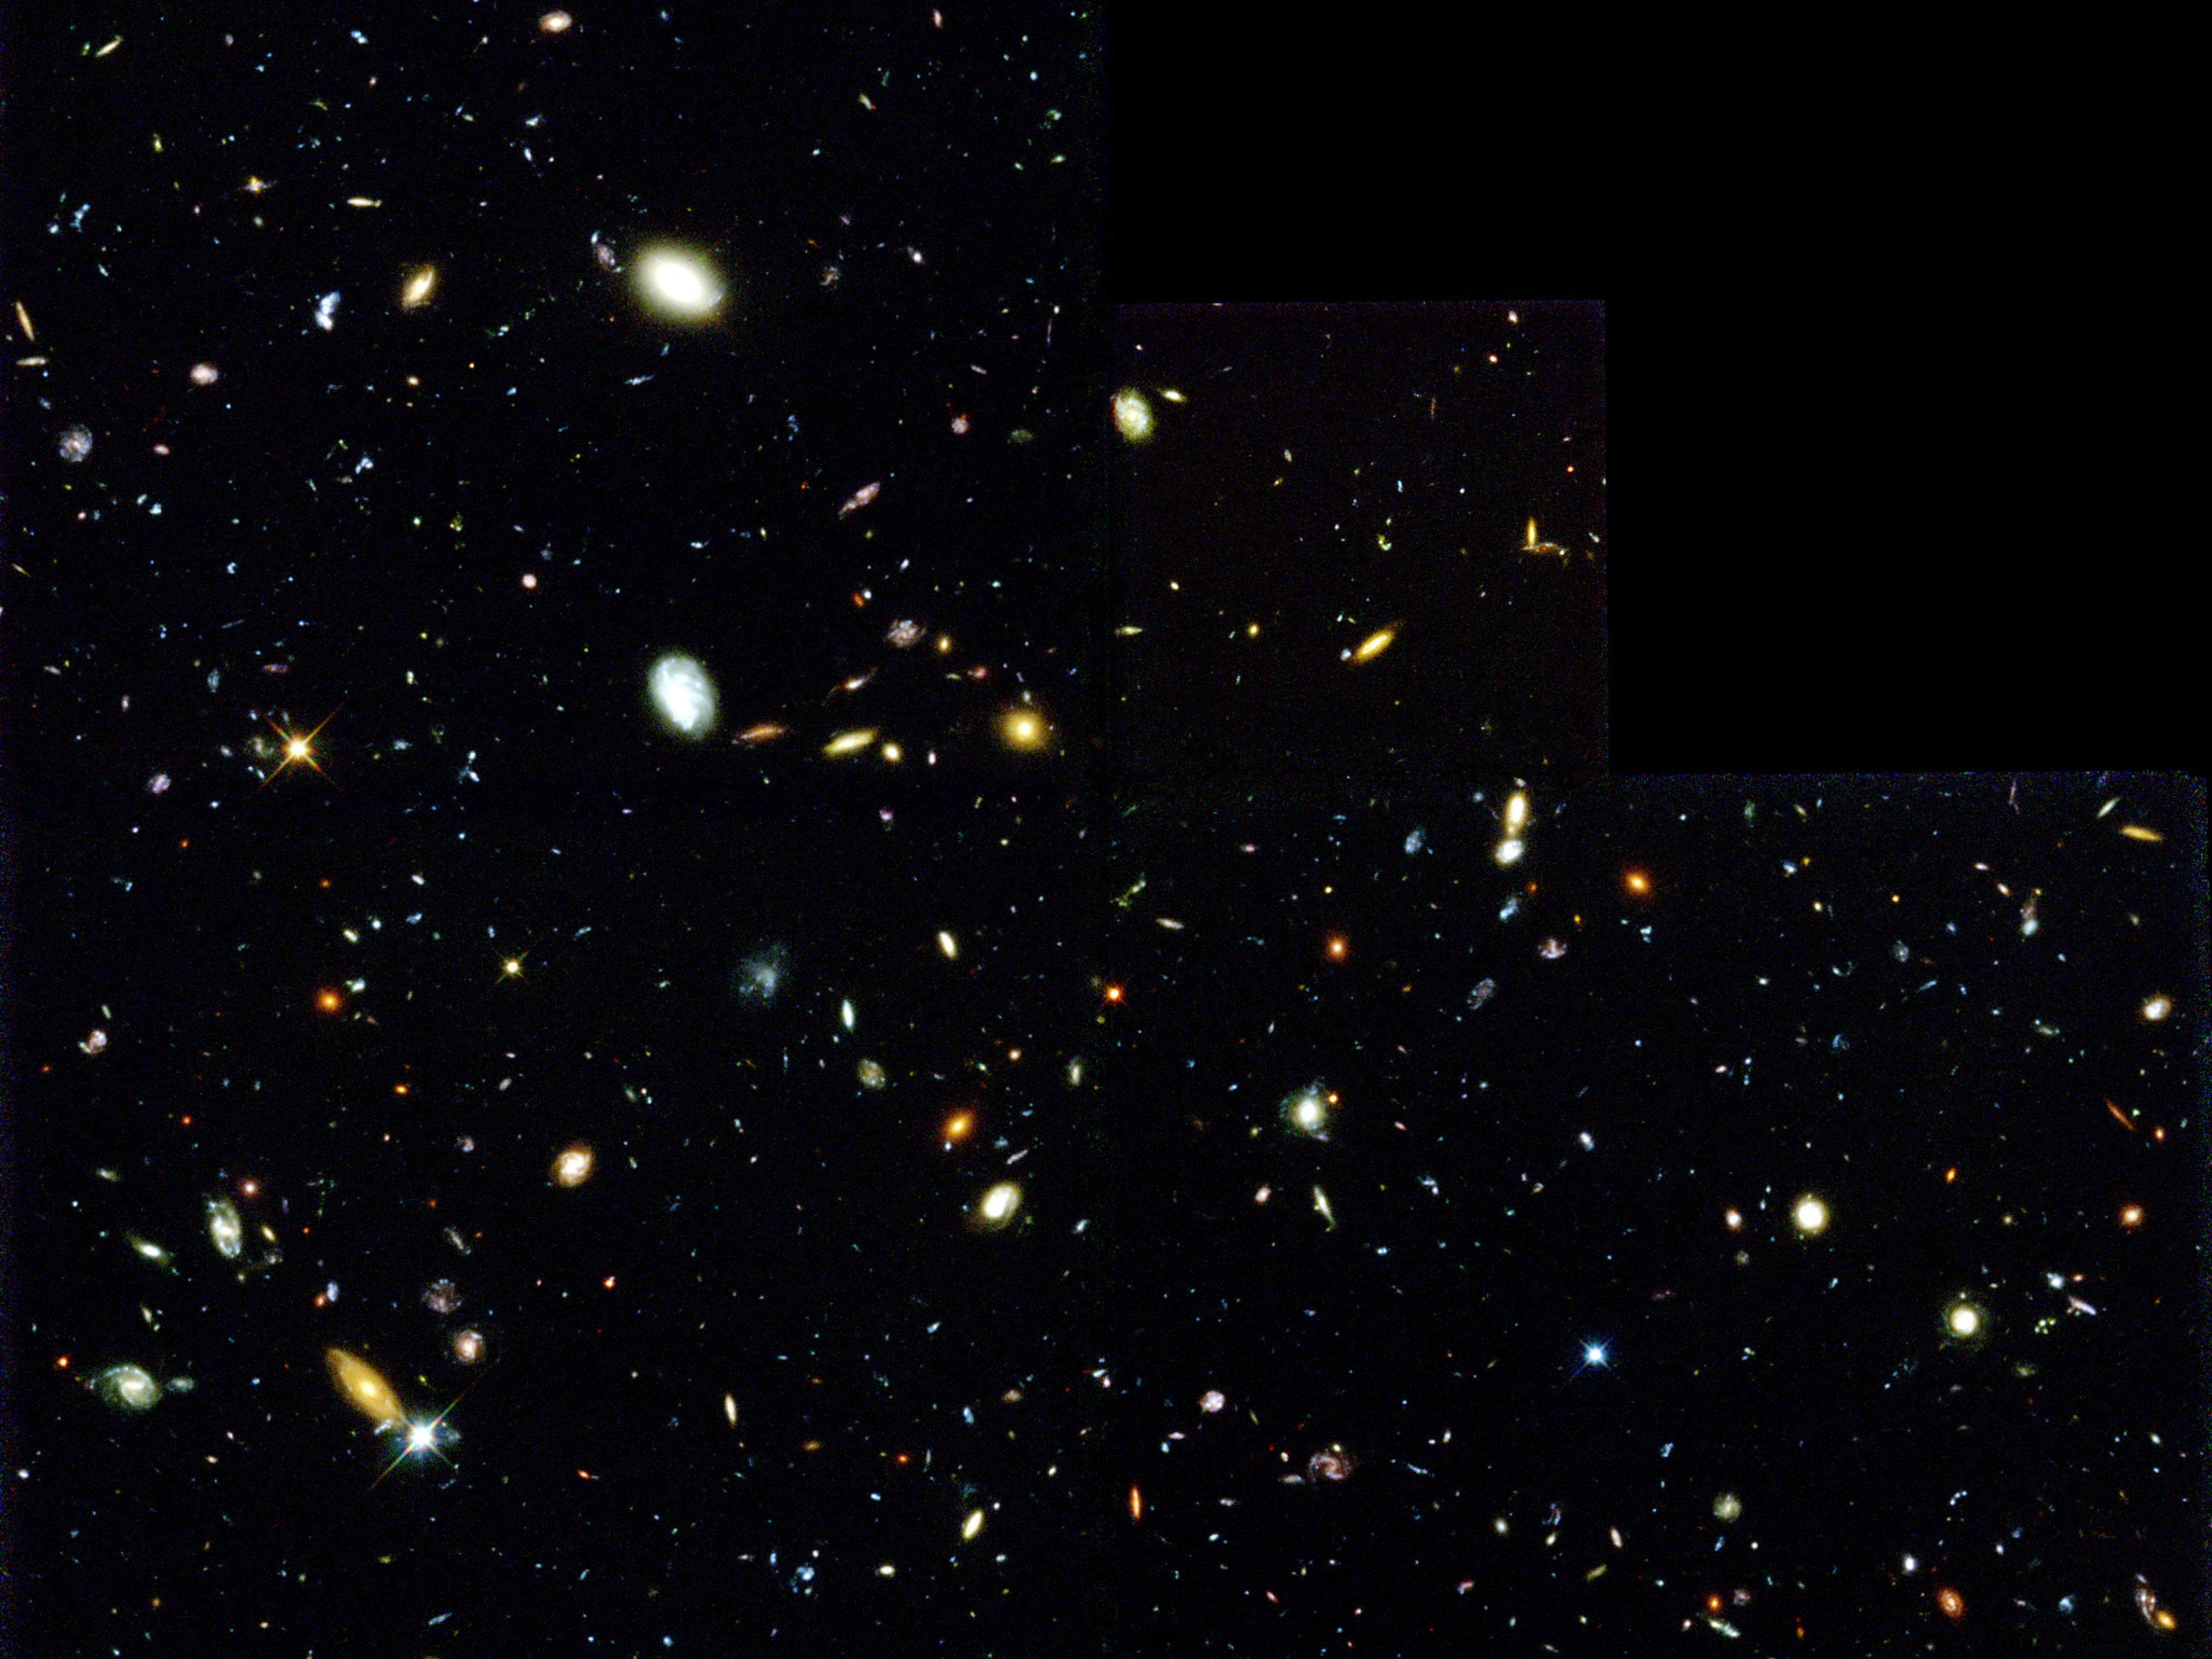
\includegraphics[width=0.9\columnwidth]{Figures/hubble_deep_field.pdf}
	\caption[Hubble Deep Field as captured by the \textit{Hubble Space Telescope}]{The Hubble Deep Field as captured by the Wide Field and Planetary Camera 2 onboard the \textit{Hubble Space Telescope} in 1995 (\citealt{Williams_1996}).}
	\label{fig:hubble_deep_field}
\end{figure}

\section{Galaxy Formation and Evolution}

To answer the questions we have about the evolution of galaxies, we must first make some inferences about the cosmology of the Universe. Our understanding of the cosmic history of galaxies is dependent on our choice of cosmology, which is widely accepted to be the $\Lambda$-CDM model (\citealt{Peebles_1980}). In this cosmology, Cold Dark Matter, matter of unknown origin, dominates over ordinary baryonic matter; and with dark energy, constitute a combined $\sim 95\%$ of the total cosmic energy budget (\citealt{Fukugita_2004}). The presence of dark matter is only evident in its gravitational interactions with matter, but can be inferred from as early as the \textit{surface of last scattering} where it can be seen that the gravitational lensing effect of large-scale distributions of matter led to distortions imprinted in the temperature and density of the cosmic microwave background (CMB). The dark energy in the Universe is parameterized in the form of the cosmological constant, $\Lambda$, which is required to explain the accelerating expansion of the Universe. In this model, galaxy formation is seeded by small quantum fluctuations in the density of the early Universe, which grow with inflation to form small overdensities that later become the sites of dark matter halos by gravitationally attracting nearby dark matter. The first galaxies formed from these originally minute overdensities. Cold dark matter cosmologies favour a \textit{hierarchical model}, where galaxies at later times formed from the coalescence of smaller, gas rich galaxies - leading to a \textit{bottom-up} theory of structure formation. As we shall show in Chapter \ref{chapter:Radio_Identifications}, this model of evolution may not explain the stellar build up of all galaxies.

\subsection{Classification of Galaxies}

The first step in understanding galaxy evolution from direct observations of galaxies across cosmic time, is to classify these galaxies according to their observable properties. Generally, galaxies can be classified into two broad groups based on their morphology: spirals and ellipticals. This dichotomy prompted the first classification scheme by Edwin Hubble (Figure \ref{fig:hubble_tuning_fork}; \citealt{Hubble_1936}), the \textit{Tuning Fork}, which shows elliptical galaxies along the handle, becoming more oblate towards the spiral galaxies. The spiral galaxies themselves are split into two categories forming the two prongs, depending on the presence of a bar at the center. At the join of the two, classified on the \textit{Tuning Fork} as S0, is where we locate \textit{lenticular galaxies}, that are recognized by their large disks, like spirals, but without the presence of arms. In the rest of this Thesis we shall predominantly be referring to elliptical galaxies as \textit{early-type galaxies} (ETGs) and spiral-like galaxies as \textit{late-type galaxies} (LTGs), as is convention. Despite their names, the two do not represent a former and latter evolutionary stage of a typical galaxy, and is rather a misnomer. A minority of galaxies do not conform to this dichotomous image and are typically grouped together as \textit{irregular galaxies}.

\begin{figure}
    \centering
	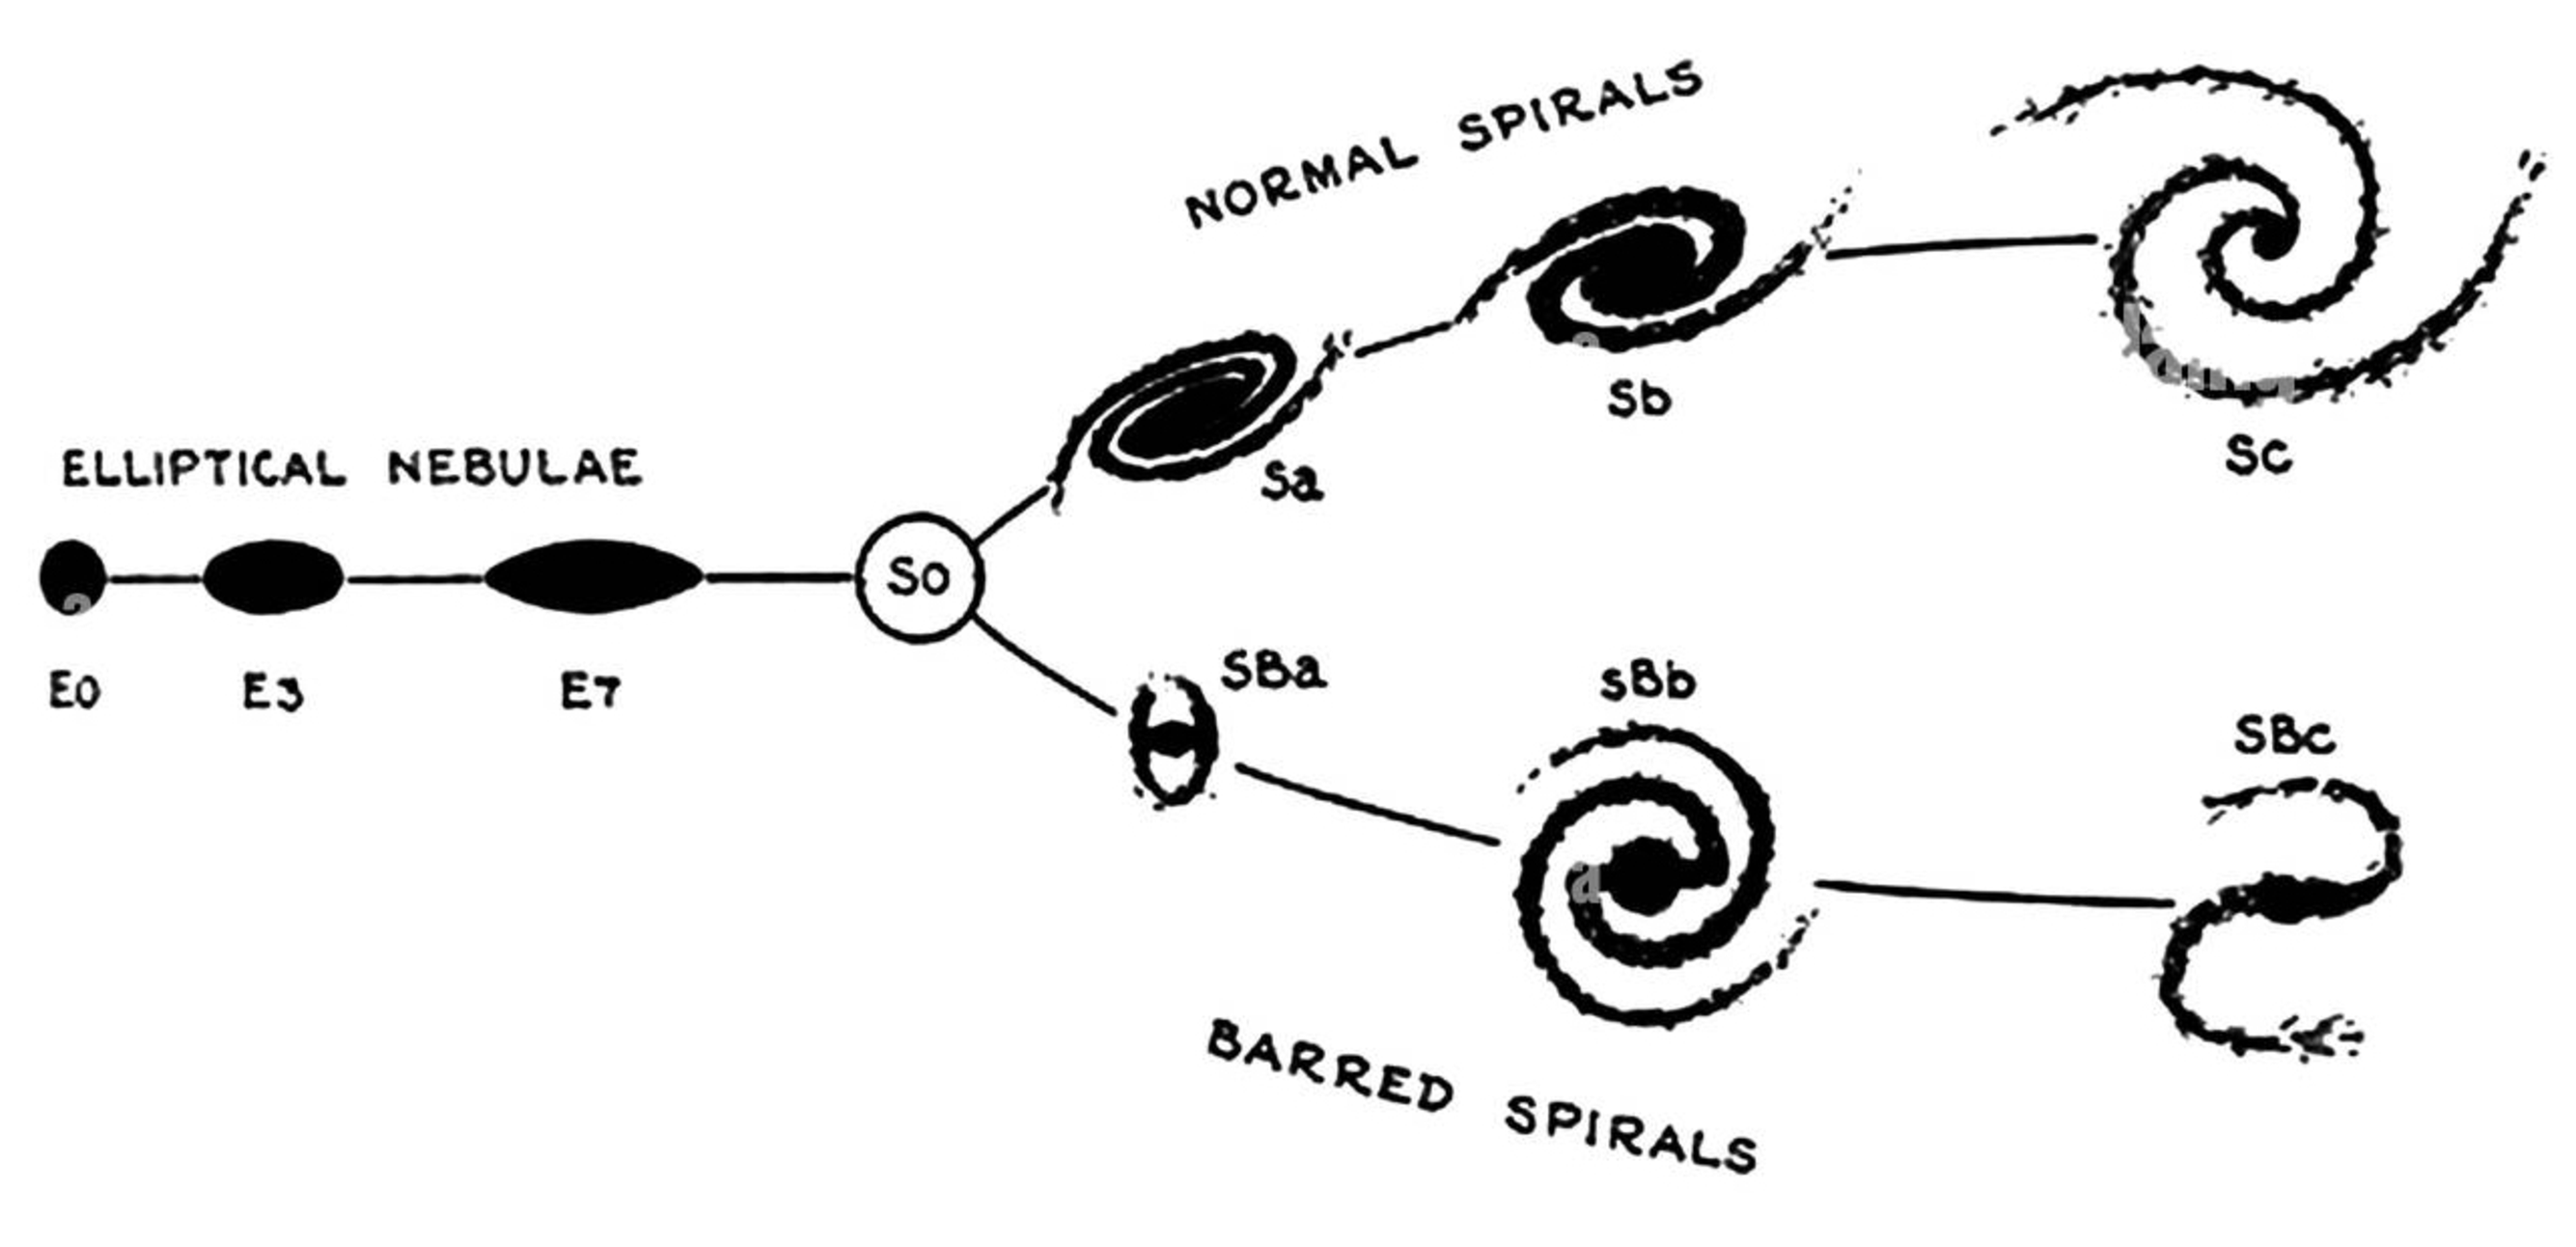
\includegraphics[width=0.9\columnwidth]{Figures/hubble_tuning_fork.pdf}
	\caption[The \textit{Hubble Tuning Fork}]{The \textit{Hubble Tuning Fork}, or the \textit{Sequence of Nebular Types} as named in \citealt{Hubble_1936}, showing spiral galaxies along the prongs of the tuning fork and elliptical galaxies along the handle. The two prongs separate those spiral galaxies with barred central bulges from those that do not. Lenticular galaxies can be found at the join of the handle to the prongs. From left to right, the elliptical galaxies become more oblate and the spiral galaxies have spiral arms that become less tightly wound around the central bulge.}
	\label{fig:hubble_tuning_fork}
\end{figure}

Beyond their shape, the two broad groups, ETGs and LTGs, have a number of physical characteristics that are common to galaxies within each class. First, the stellar populations of ETGs and LTGs are different. ETGs are dominated by old stellar populations that appear red in colour because they contain longer-lived, low mass stars, whereas LTGs typically have younger stellar populations of massive, but very short-lived stars. ETGs are considered to be some of the most massive, luminous galaxies (due to having vast quantities of old stars) observed in the local Universe (\citealt{Bernardi_2003, Kelvin_2014, Moffett_2016}). They are spheroidal in shape with a central bulge of stars where most of the interstellar medium (ISM) is located, though it is not expected to be substantial, and the limited amount of gas in the ISM restricts the level of new star formation. In a hierarchical view of star formation, such ellipticals are formed from a series of major and minor mergers that consume the gas in the galaxy, leading to the quiescent systems observed today (\citealt{Toomre_1972}). In contrast, LTGs have dusty spiral arms with sites of active star formation, with older stars mainly located within the central bulge. While ETGs are largely devoid of gas, LTGs have a rich ISM that continues to fuel star formation, creating new stars at typical rates of a few stars per year (\citealt{Kennicutt_1983, Gao_2004}). Our own Milky Way is an SBc spiral galaxy (\citealt{Gerhard_2002}) with active star formation at a rate of $\sim 2\,M_\odot$yr$^{-1}$ (\citealt{Noriega-Crespo_2013, Licquia_2015, Elia_2022} and references therein).

\subsection{The Star Forming Main Sequence}
\label{sec:star_forming_main_sequence}

A natural diagram to illustrate the difference in the colour of ETGs and LTGs is to plot the colours of optically-selected galaxies against their absolute magnitude. Galaxies discovered in optical surveys readily form two distinct regions: a \textit{red sequence} and a \textit{blue cloud}, with a sparsely populated region in between - the \textit{green valley}. Due to their very different optical colours, the red sequence is dominated by ETGs and the blue cloud dominated by LTGs. Moving away from observed quantities to intrinsic quantities, we note that the colour is a strong indicator of the star formation rate (SFR) in a galaxy and that absolute magnitude is approximately proportional to the size of the stellar population, and thus the stellar mass, $M_*$. In this formalism, the blue galaxies form a tight correlation known as the \textit{Main Sequence} (MS) or \textit{Star Forming Main Sequence}, while the red sequence now occupies a \textit{passive cloud} (or "red and dead" or "quiescent") region that lies below the MS at lower star formation rates (\citealt{Noeske_2007, Daddi_2007, Elbaz_2007, Rodighiero_2011}). Figure \ref{fig:star_forming_main_sequence} shows the main sequence and passive clouds (grey contours) that form from the optically-selected Sloan Digital Sky Survey (SDSS; \citealt{York_2000}). Additionally, \citealt{Saintonge_2017} present the \textit{Extended CO Legacy Database for GASS}, xCOLD GASS, a mass-selected sample from SDSS that have molecular gas mass estimates, which are overplotted in colour in Figure \ref{fig:star_forming_main_sequence}. The molecular gas mass fraction, $f_{\textrm{H}_2} \equiv M_{\textrm{H}_2}/M_*$, clearly declines towards the passive cloud, showing the depleted amount of gas in ETGs.

\begin{figure}
    \centering
	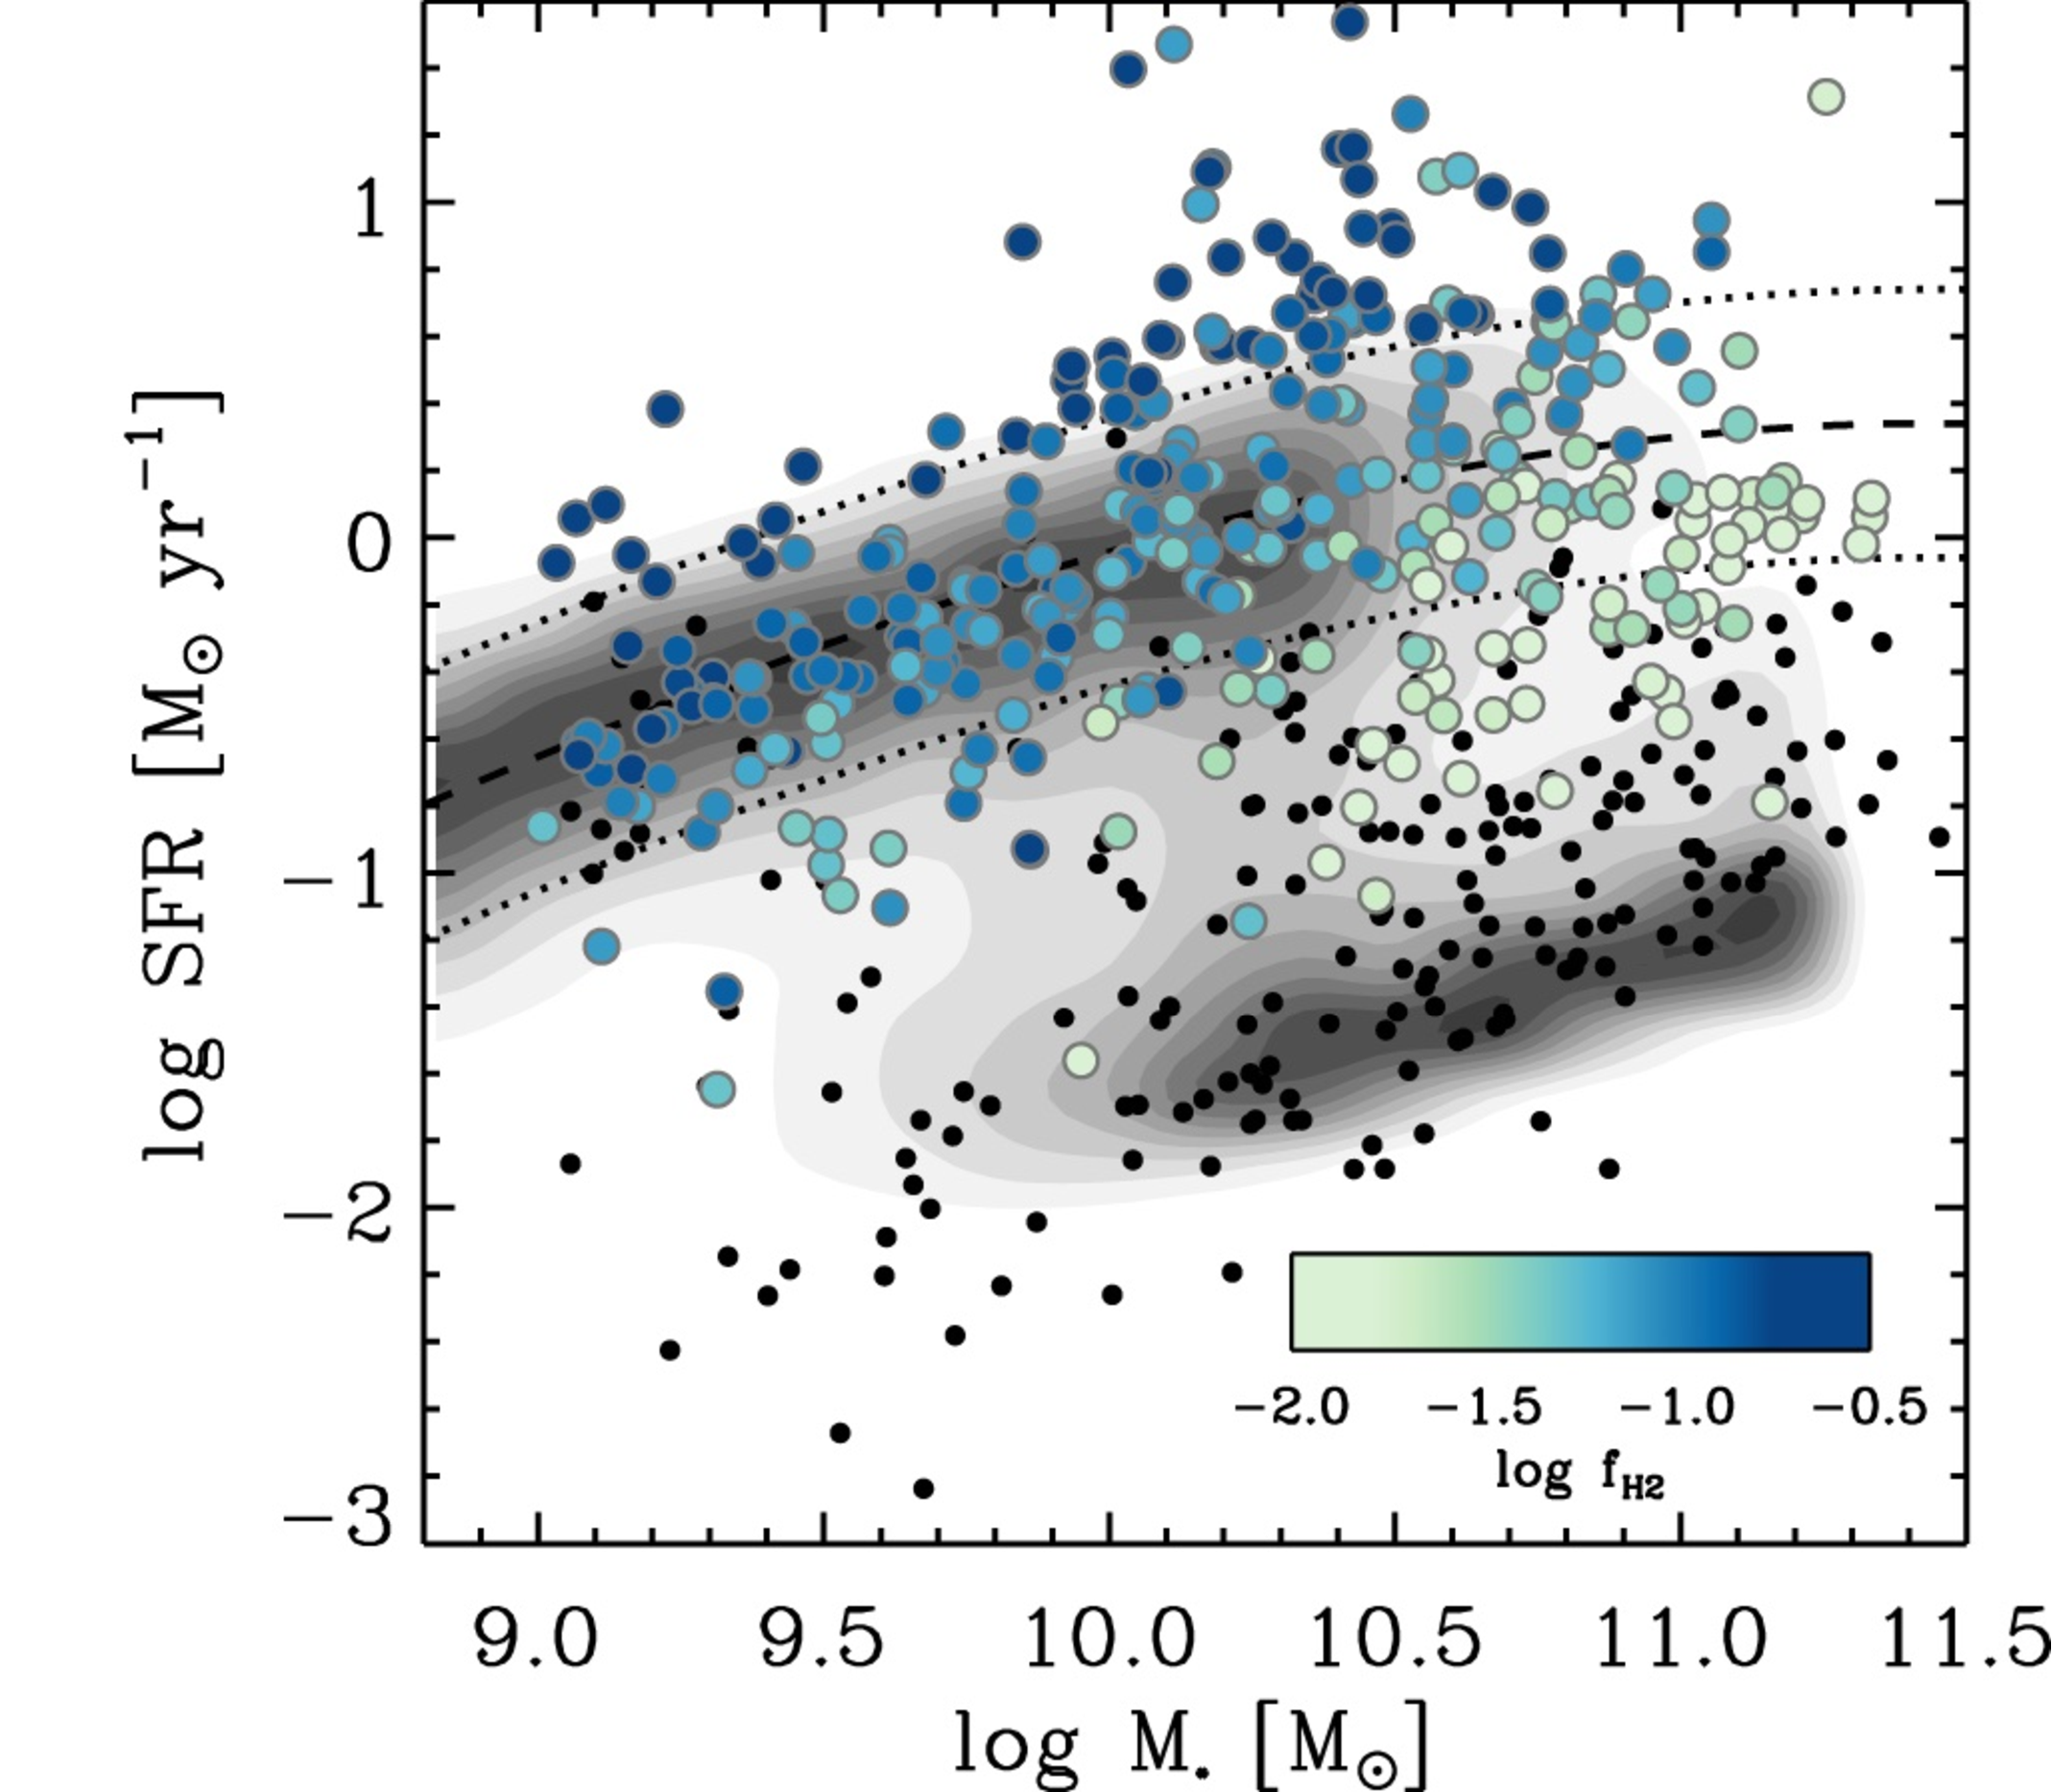
\includegraphics[width=0.8\columnwidth]{Figures/saintonge_ms.pdf}
	\caption[The distribution of SDSS galaxies in the SFR-$M_*$ plane]{The distribution of SDSS galaxies in the SFR-$M_*$ plane (grey contours) from \citealt{Saintonge_2017} (Figure 8). The dashed line represents the location of the main sequence, while the dotted lines represent $\pm0.4\,$dex scatter around this relationship. The coloured points show the distribution of galaxies from xCOLD GASS, coloured according to their molecular gas mass fraction. The black points are galaxies without detected CO (1 - 0) emission lines, as used to measure the mass of molecular gas.}
	\label{fig:star_forming_main_sequence}
\end{figure}

It is predicted that the vast majority, approximately $90\%$, of all cosmic star formation between redshifts $0$ and $2.5$ occurs in galaxies that reside on the MS (\citealt{Rodighiero_2011, Sargent_2012}), however, we also know that an important contribution comes from galaxies that sit substantially above this relation. These galaxies, undergoing high levels of star formation for a short period of time, are collectively referred to as \textit{starburst galaxies} (e.g. \citealt{Muxlow_2006, Rinaldi_2022}). Starbursts\footnote{Unfortunately, there is yet to be a population of galaxies referred to as \textit{Opal Fruits}.} form a small minority of galaxies, approximately $2\%$ of star forming galaxies depending on the exact definition of a starburst, but contribute $\sim 10\%$ of the cosmic star formation rate density (SFRD) at $z \sim 2$ (\citealt{Rodighiero_2011}), corresponding to the time in cosmic history when star formation was at its peak (see Section \ref{sec:cosmic_star_formation_history}).

Given that galaxies in the passive cloud have large stellar masses, they must have been at some point among the actively star forming galaxies, following which some process quenched them of their star formation leading them to the passive cloud. The prevailing interpretation of the SFR-$M_*$ diagram is that a typical galaxy evolves along the sequence, gaining stellar mass, increasing their star formation rate accordingly, and depleting the gas available for star formation in the process. At some point, the galaxy stops forming stars entirely, and falls off the main sequence. The valley between the MS and the passive cloud, a result of a dearth of galaxies in this regime, suggests that the quenching process that turns off the star formation in the galaxy is fast. This image of galaxy evolution, however, is not without scepticism. Recent studies \mbox{(e.g. \citealt{Eales_2018a, Bremer_2018, Phillipps_2019})} have suggested that the bimodal distribution of star forming and passive galaxies may be a reflection of selection effects in optical surveys, prompting attempts to define the whole population of galaxies using a single distribution (e.g. \citealt{Corcho-Caballero_2020}). The evidence given in \citealt{Eales_2018a} is that samples that are instead selected in sub-mm surveys occupy this middle ground, forming a \textit{green mountain}. On the basis that the whole galaxy population falls on a singular curved Galaxy Sequence, the sub-mm will naturally pick out galaxies with high sub-mm/optical luminosity ratios due to Malmquist bias, which lie at the "knee" of this distribution. In the reverse scenario, theses galaxies will be underrepresented in an optically selected sample, worsening the appearance of the green valley. Further evidence of a possible single sequence comes from the observation that morphological class gradually changes along this sequence (\citealt{Eales_2018b}).

Whether there are two distinct classes or not, some physical process must be converting a star forming galaxy on the MS to one that is passive, quenching it of star formation. There are many possibilities that have been proposed as the cause of quenching, and it is likely that all are important in some regard. These processes include, but may not be limited to: stellar feedback and winds from supernovae removing the gas from a galaxy (\citealt{Hayward_2017}); gas expulsion by active galactic nuclei (AGN; \citealt{Springel_2005, Croton_2006, Cicone_2014, Harrison_2017}); the formation of a galactic bar or central bulge (\citealt{Bournaud_2007, Martig_2009}) which relocates the gas to the galactic center and reduces the star formation in the disk; a range of environmental processes such as galaxy merging (\citealt{Lavery_1994, Weigel_2017}) which ignites a starbursting phase that rapidly consumes the gas; ram-pressure stripping, the loss of gas as the galaxy passes through the intra-cluster medium (\citealt{Gunn_1972, Boselli_2006, Domainko_2006, Boselli_2014}), and quenching mechanisms that result from being in high density environments, like galaxy harassment and strangulation (\citealt{Moore_1996, Moore_1998, Bekki_2002}).

\subsection{Cosmic Star Formation History}
\label{sec:cosmic_star_formation_history}

We have seen that the star formation rates of galaxies are intrinsically linked to their evolutionary stage, and thus it is unsurprising that we identify an evolution in the integrated SFRs of galaxies with cosmic time. By measuring the star formation of many galaxies at different epochs, we can build a picture of the star formation density in the Universe. The cosmic history of star formation is one of the fundamental observables of astronomy, giving us an insight into the timeline for which gas forms into stars, heavy elements are produced (elements heavier than the primordial hydrogen and helium are produced in stars), and dust is formed (as dust is a natural byproduct of star formation, see Section \ref{sec:lifecycle_of_dust}).

The cosmic star formation rate density in the Universe is straightforwardly estimated from the star formation rates of galaxies based on their rest frame UV photometry. The UV maps the light from hot, young, massive stars and therefore directly traces recent star formation (e.g. \citealt{Madau_1996, Lilly_1996, Wyder_2005, Schiminovich_2005, Dahlen_2007, Reddy_2009, Robotham_2011, Cucciati_2012, Schenker_2013, Finkelstein_2015}). However, we also note that approximately half of all optical and UV light from stars ever emitted in the Universe has been absorbed by dust and re-emitted at far-infrared (FIR) and sub-millimeter (sub-mm) wavelengths (\citealt{Puget_1996, Fixsen_1998, Dole_2006, Driver_2008, Driver_2016}). This means that a significant contribution to the SFRD is hidden behind dust and must be determined from far-IR/sub-mm indicators of star formation that probe the stellar light reprocessed by dust (e.g. \citealt{Magnelli_2011, Casey_2012, Magnelli_2013, Gruppioni_2013, Swinbank_2014, Bouwens_2016, Bourne_2017, Koprowski_2017, Novak_2017, Liu_2018, Bouwens_2020, Dudzeviciute_2020}).

Figure \ref{fig:cosmic_sfrd} shows that the dust-obscured and unobscured measures of the SFRD have peaks at $z\sim2$ (when the Universe was roughly $3$ billion years old), followed by a slow decline by a factor of $\sim 8$ to the present day. The short period corresponding to the peak of star formation is often referred to as \textit{cosmic noon}. In the approximate $3.5\,$Gyr between $z\sim3$ and $z\sim1$, spanning cosmic noon, up to half of the stellar mass we observe today was formed (\citealt{Forster-Schreiber_2020}). The galaxies that are identified at these redshifts are ideal targets for tracing the formational epoch of the massive LTGs and ETGs seen in the local Universe. We see that most of the star formation at $z < 3$ is obscured by dust and even at higher redshifts the contribution still appears significant. The FIR and sub-mm traced component has dominated the cosmic history of star formation for the past $\sim 12\,$Gyr, contributing approximately $80\%$ of the total star formation. The top panel of Figure \ref{fig:cosmic_sfrd} shows the contribution from galaxies with different IR luminosities to the dust-obscured star formation. It is clear that massive, IR luminous galaxies dominate the star formation history at earlier times. It is such galaxies, that appear particularly bright at far-IR wavelengths, that are crucial for our understanding of obscured star formation. 

At this point, we clarify some acronyms commonly used to refer to bright infrared galaxies that will be referred to throughout the Thesis (the IR luminosities of galaxies are assumed to be the bolometric luminosity integrated between $8$ and $1,000\,\mu$m in the rest frame):

\begin{itemize}
    \item Luminous Infrared Galaxy (LIRG: $10^{11} < L_\textrm{IR} [L_\odot] < 10^{12}$).
    \item UltraLuminous Infrared Galaxy (ULIRG: $10^{12} < L_\textrm{IR} [L_\odot] < 10^{13}$).
    \item HyperLuminous Infrared Galaxy (HyLIRG: $L_\textrm{IR} [L_\odot] > 10^{13}$).
\end{itemize}

\begin{figure}
    \centering
	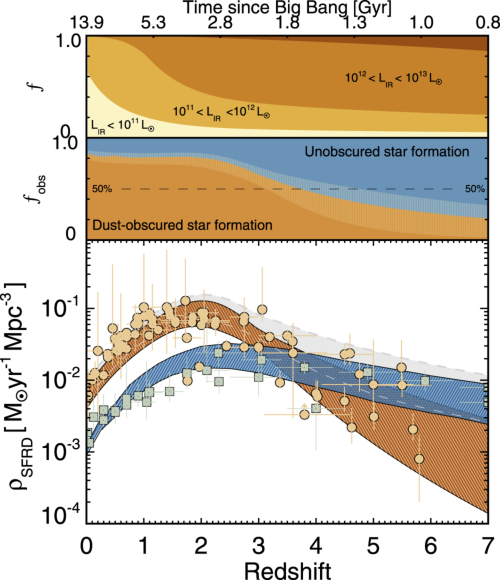
\includegraphics[width=0.8\columnwidth]{Figures/cosmic_sfrd.pdf}
	\caption[Cosmic star formation history]{The cosmic star formation history from \citealt{Zavala_2021}. Contributions to the total star formation rate density (grey) from dust-obscured IR/sub-mm surveys and from unobscured UV/optical surveys are shown in orange and blue, respectively. The top panel shows the relative contribution to the dust-obscured SFRD from galaxies with different IR luminosities. The middle panel represents the fraction of SFRD that is dust-obscured.}
	\label{fig:cosmic_sfrd}
\end{figure}

Looking back to cosmic noon, much of the star formation within dusty galaxies is happening in ULIRGs, while the integrated dust-obscured star formation begins to fall. This suggests that the number of massive galaxies declines at higher redshifts, but their individual contribution becomes more important. Particularly at high redshifts ($z \gtrsim 3$), the exact amount of dust-obscured star formation is still uncertain and large samples of galaxies with measured dust emission are therefore required to elucidate our view on the cosmic history of star formation.

\section{The Interstellar Medium}

The interstellar medium (ISM) refers to the matter that fills the space in between the stars of a galaxy. It is the medium in which stars are born, and latter replenished with enriched material when they die. The matter comes in the form of gas - in ionic, atomic and molecular forms - and dust, in overwhelming favour of gas which constitutes $\sim99\%$ of the ISM, and dust the other $1\%$ (\citealt{Ferriere_2001}). By mass, the gas in the ISM is around $70\%$ hydrogen, $28\%$ helium and $2\%$ heavier elements, reflecting only a small change from the ratios of the primordial matter created after the Big Bang (\citealt{Klessen_2016}). In terms of volume, most of the ISM is occupied by ionized gas, but due to its incredibly low volume density, only accounts for around $25\%$ of the gas mass. Most of the gas mass in a galaxy is in the form of neutral atomic gas (H and He) or molecular gas (H$_2$) found in dense clouds that take up only $1 - 2\%$ of the total volume of the ISM (\citealt{Dyson_1997, Klessen_2016}).

The ISM spans a wide range of temperatures and densities, leading to many models of the ISM being in distinct phases, despite there being no obvious separation between them (\citealt{Cox_2005}). A two phase model was first proposed by \citealt{Field_1969}, showing that atomic gas in the ISM can exist at two stable temperatures. These two solutions correspond to cold and dense gas at $T\sim100\,$K and warm, diffuse gas at $T\sim10^4\,$K. These are now referred to as the Cold Neutral Medium (CNM) and Warm Neutral Medium (WNM), respectively. This model was extended to three phases by \citealt{McKee_1977}, who noted that supernovae in the ISM creates bubbles of very hot, ionized gas ($T\sim10^6\,$K). This phase of the ISM is known as the Hot Ionized Medium (HIM). A cooler, Warm Ionized Medium (WIM) has a temperature and density similar to the WNM, but contains around $90\%$ of the ionized gas in the ISM (\citealt{Haffner_2009}). A final distinction is typically made for the molecular clouds that are cold, but distinctly more dense than the CNM. These molecular gas clouds have a range of masses and sizes, and their location are known to correlate with observed star formation in the Galaxy. The approximate temperatures, densities, mass fractions and volume filling fractions of each phase in the ISM for a dynamic spiral galaxy are given in Table \ref{tab:ISM_phases}. The fractions are highly uncertain but represent what might be realistic estimates for a spiral galaxy containing all five phases of this interpretation of the ISM. This multi-phase picture is certainly an oversimplification of the conditions found in the ISM. The ISM is shaped by a variety of processes that blur the distinction between these phases, such as turbulence from supernova shocks (\citealt{MacLow_2004}) and stellar winds, thermal instability (\citealt{Kritsuk_2002}) and the presence of magnetic fields. The actual ISM in a galaxy is continuous and dynamic with transitional regions.

\begin{table}
	\centering
	\begin{tabular}{p{4cm}|p{2.5cm}|p{2.75cm}|p{1.5cm}|p{2cm}}
		\hline
		\hline
		Phase & T [K] & $n$ [atoms cm$^{-3}$] & $f_{\textrm{Mass}}$ & $f_{\textrm{Volume}}$ \\
		\hline
		\hline
		Molecular Clouds & $10 - 20$ & $>10^2$ & $\sim 20\%$ & $<1\%$ \\
		Cold Neutral Medium & $50 - 100$ & $20 - 50$ & $\sim 40\%$ & $\sim2 - 4 \%$\\
		Warm Neutral Medium & $(6 - 10)\times10^3$ & $0.2 - 0.5$ & $\sim 30\%$ & $\gtrsim 30\%$ \\
		Warm Ionized Medium & $\sim8\times10^3$ & $0.2 - 0.5$ & $\sim 10\%$ & $\gtrsim 15\%$ \\
		Hot Ionized Medium & $\sim10^6$ & $\sim10^{-2}$ & $\sim 1\%$ & $\lesssim 50\%$ \\
		\hline
	\end{tabular}
	\caption[The temperatures, densities, mass and volume filling factors of ISM phases]{The different phases of the ISM and their expected temperatures, densities, mass fractions and volume filling factors, as tabulated in \citealt{Ferriere_2001}.}
	\label{tab:ISM_phases}
\end{table}

Figure \ref{fig:interstellar_medium} shows various components of the ISM in the Galaxy, as traced by different wavelengths of the electromagnetic spectrum. The top two panels highlight the starlight that is observable at optical ($0.5\,\mu$m) and near-infrared ($2\,\mu$m) wavelengths. The stellar light is blocked by dust in the optical image, whereas the near-infrared clearly shows the stellar distribution, making the dark dust clouds appear almost transparent. The benefit that the infrared provides in identifying the stellar light of a galaxy, compared to optical wavelengths, is a key motive for the studies presented in Chapters \ref{chapter:Data_Release_3} and \ref{chapter:Dust_Mass_Functions}. As we traverse the electromagnetic spectrum to the thermal peak in the far-infrared (third panel, observed at $350\,\mu$m) the emission from the dust itself becomes visible. The final three panels show the emission from atomic, ionized and molecular gas in the Galaxy. The atomic gas is traced by the $21\,$cm spectral line, originating from the hydrogen \textit{spin-flip} transition between a proton-electron aligned state to an anti-aligned state. This transition is forbidden - the mean lifetime of a hydrogen atom being in the excited, aligned state is approximately $11$ million years (\citealt{Mhaske_2022}) - meaning that the likelihood of the transition is incredibly rare. However, as can be seen in the figure, the abundance of atomic hydrogen means that the $21\,$cm line is still a useful tracer for gas in the ISM. The limitation of the $21\,$cm line is that it is only useful for tracing the distribution of neutral hydrogen in the local Universe where the emission is strong enough to be detected. The $74\,$cm radio emission in the penultimate panel traces the radiation from ionized gas. The radio emission emanates from accelerated charged particles, which may be observed in HII regions and supernova remnants. The final panel shows the molecular gas phase, as traced by the $2.6\,$mm spectral line of carbon monoxide (CO). As will be detailed later, the rotational transitions of the CO molecule is a useful tracer of dense molecular regions, and it is often assumed that wherever there are CO molecules there must also exist H$_2$ molecules. This map therefore shows the locations of cold gas in the Galaxy and the sites of star formation.

\begin{figure}
    \centering
	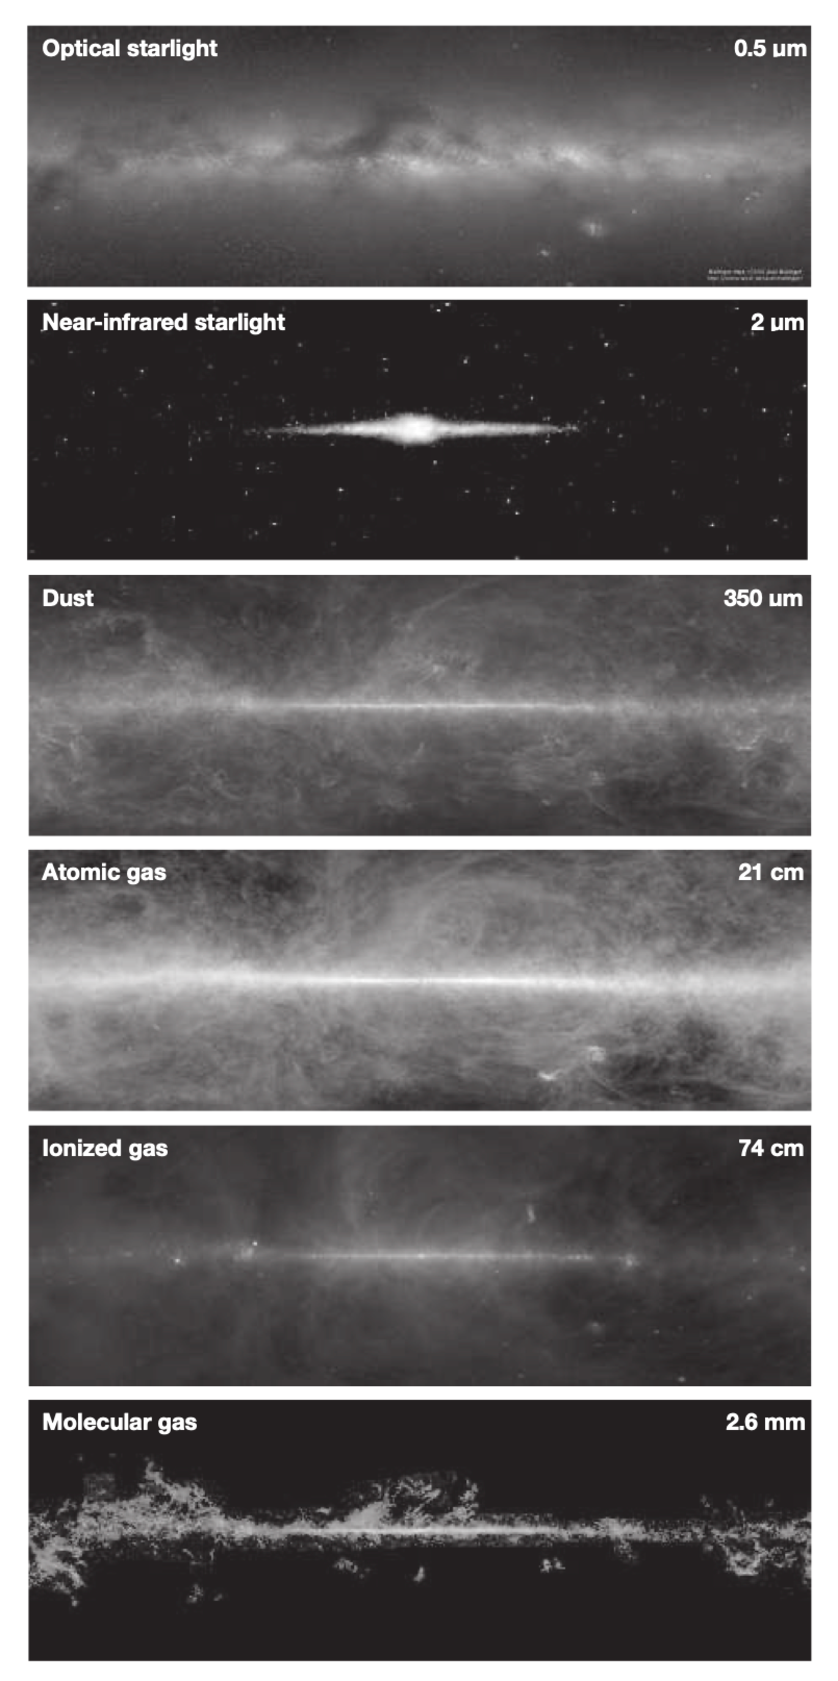
\includegraphics[width=0.75\columnwidth, height=0.92\textheight]{Figures/interstellar_medium.pdf}
	\caption[The plane of the Galaxy observed at various wavelengths]{The plane of the Galaxy observed at different wavelengths as presented in \citealt{Williams_2021}. From top to bottom the panels show: the optical starlight at $0.5\,\mu$m; the near-infrared starlight at $2\,\mu$m; the interstellar dust at $350\,\mu$m; the atomic gas at $21\,$cm; the ionized gas at $74\,$cm and the molecular gas at $2.6\,$mm.}
	\label{fig:interstellar_medium}
\end{figure}

\section{Cosmic Dust}

\subsection{Chemical Composition of Dust}

Cosmic dust is a general term that refers to the solid particles that exist in the ISM. These interstellar grains can have a range of sizes between $\sim 10\,$nm and $\sim 1\,\mu$m (\citealt{Kim_1994, Galliano_2018}) and are mostly composed of carbonaceous materials (materials that are predominantly Carbon by mass) and silicates. The larger dust grains are primarily silicates and amorphous carbon, which are prime candidates for the dust grains that absorb UV and optical starlight and reradiates this energy in the far-IR and sub-mm regimes. Hydrogenated carbonaceous materials, like Polycyclic Aromatic Hydrocarbons (PAHs), are chemical compounds formed of carbon and hydrogen molecules and are also an important component of interstellar dust grains. These molecules are the cause of strong spectral lines that can be observed in the mid-infrared (\citealt{Tielens_1987, Draine_2007a, Draine_2007b}).

\subsection{The Reprocessing of Starlight}

The presence of dust along the line of sight to a population of stars can have several consequences on the emission that is observed. First, if the dust is thick enough, any background stellar light may not be visible at all, as is the case with some dark nebulae in the Galaxy such as the \textit{Horsehead Nebula} (\citealt{Greenberg_2002}). For less opaque dust clouds, the light passing through can be dimmed due to the effects of dust extinction. This refers to the amount of background light that is absorbed and scattered out of the line of sight to the observer. The dimming effect is dependent on several factors including the density of the dust cloud, the grain size distribution and the wavelength of the light. More generally, dust attenuation refers to the effect on the spectrum of a background object as a result of dust, which includes dust extinction, but also includes scattering back into the line of sight and the light from unobscured stars. It is the attenuated stellar emission that is observed as a strong peak in the far-IR region of a galaxy's spectral energy distribution (SED). Figure \ref{fig:unattenuated_attenuated_sed} shows the UV to far-IR SED of NGC 337, modelled using \texttt{MAGPHYS} (\citealt{daCunha_2008}), which illustrates how the true stellar spectrum of a galaxy (blue) is attenuated by dust to produce the far-IR emission (green) and the observed UV to far-IR spectrum (black). Moreover, interstellar dust is more efficient at absorbing and scattering blue light compared to red light, due to its shorter wavelength corresponding to the typical size of abundant small grains, meaning that background stars behind a cloud of dust often appear more red than they really are. This effect is known as dust reddening and can be observed in the spectrum of NGC 337 - the shorter the wavelength (towards the blue end of the spectrum), the greater the difference between the attenuated and unattenuated stellar spectra.

\begin{figure}
    \centering
	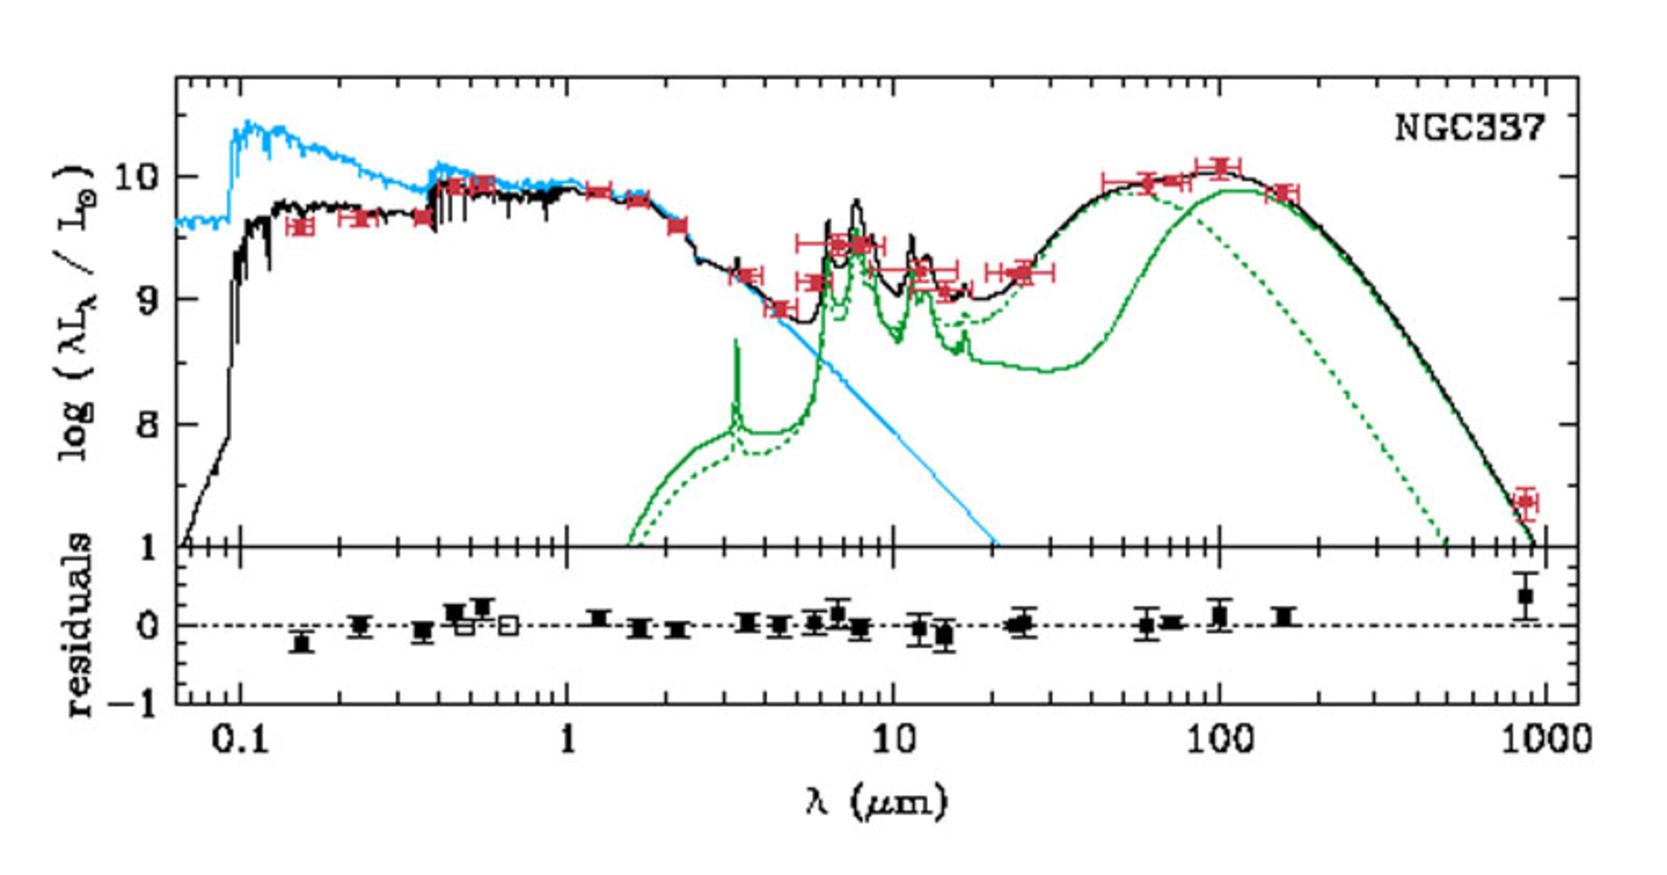
\includegraphics[width=0.9\columnwidth]{Figures/unattenuated_attenuated_sed.pdf}
	\caption[SED of NGC 337]{The best fitting SED model to the observed spectra of NGC 337 adapted from \citealt{daCunha_2008}. The blue line represents the unattenuated stellar spectrum and the green lines show the reprocessed light by dust, separated into dust in the diffuse ISM (solid) and dust in molecular clouds (dotted). The attenuated (observed) SED from the UV to far-IR is shown as the black line, which is fitted to the data points (red).}
	\label{fig:unattenuated_attenuated_sed}
\end{figure}

A fundamental assumption that is made throughout this Thesis is that we can trace the hidden star formation in a galaxy via the dust emission observed in the far-IR and sub-mm wavelengths. Figure \ref{fig:interstellar_medium} shows that the dust and gas are well mixed in the ISM of the Galaxy, suggesting that interstellar dust coexists with the gas in the ISM and thus dust masses may be a useful measure of the total mass of the ISM. Moreover, because most UV emission comes from recent star formation in a galaxy, the reprocessed IR luminosity is often assumed to be directly proportional to the fraction of the energy from star formation that gets absorbed by dust. As a result, studying the emission from dust is vital in our understanding of the hidden star formation via its connection to gas, and the properties of the dust are important in our understanding of the conditions required for star formation to occur.

\subsection{The Lifecycle of Dust}
\label{sec:lifecycle_of_dust}

The lifecycle of dust grains, the mechanisms in which they are produced and destroyed, are important in understanding the metal enrichment and stellar evolution of galaxies. Dust can form in a number of ways including in the stellar winds of evolved stars, from the ejecta of supernovae or from forming in situ in the ISM (\citealt{Draine_2009}). Traditionally, the majority of dust was presumed to be formed in the outer envelopes of latter stage stars, such as red giant branch (RGB) and asymptotic giant branch (AGB) stars. These stars have masses of $1 < M_\textrm{star} [M_\odot] < 8$ and are in a late phase of evolution, having left the (stellar) main sequence and formed heavy elements via stellar nucleosynthesis. The metals solidify into grains in the envelopes of RGB and AGB stars and are carried out in into the ISM by stellar winds (\citealt{Whittet_2002}). For more massive stars with $M_\textrm{star} > 8\,M_\odot$, dust can form in the ejecta of supernovae, condensing from the leftover expanding material. The problem with this pathway, however, is that the dust yields from a single supernova are still a matter of debate, with studies observing dust masses in supernova remnants between roughly $0.05\,M_\odot$ and $1\,M_\odot$ (\citealt{Rho_2008, Dunne_2009, Barlow_2010, Matsuura_2011, Gomez_2012, Matsuura_2015, Chawner_2019}). Much of this debate stems from questions about how the dust formed in supernovae may survive the destructive shock waves that are produced (\citealt{Draine_1979, Jones_1996}). The production rate of dust is a key open question, particularly for studies in the early Universe where a \textit{Dust Budget Crisis} has been proposed (e.g. \citealt{Dwek_2007, Michalowski_2010, Valiante_2011}). This refers to the difficulty in explaining the high dust masses observed in high redshift galaxies from dust produced via the Low-Intermediate Mass Stars (LIMS). Above redshifts $\sim 5$, there is little time for significant amounts of dust to be produced from the post main-sequence evolution of LIMS (\citealt{Morgan_2003, DiCriscienzo_2013}). The final production mechanism we mention here is dust formed in situ via grain growth. This method is most effective in the dense ISM, and so is particularly important in molecular clouds. Grain growth occurs when the conditions allow for the grains to form mantles of ice, which allow metals to subsequently stick to the grains (known as \textit{coagulation}, \citealt{Blain_2004}). We have mentioned one way in which dust can be destoyed in the ISM, supernova shocks, but a second process contributing to dust destruction is \textit{sputtering}. Sputtering occurs as the result of the bombardment of gas atoms in dense environments causing the sublimation of the dust grains (\citealt{Barlow_1978, Jones_2004}). The combination of production and destruction mechanisms form a cyclical nature to dust in the ISM; dust is formed from stellar environments, they are expelled into the ISM and take an enriched form, they get incorporated into molecular clouds, which subsequently leads to star formation and the cycle repeats.

\section{Observing Dusty Star Forming Galaxies in the Far-IR and Sub-mm}

The long wavelengths covering the thermal dust emission can have several names, sometimes referred to as the far-infrared, and at other times as the sub-millimeter. While the two terms are used rather interchangeably, we shall continue with the convention that the far-infrared waveband extends from roughly $10$ to $400\,\mu$m, while the sub-millimeter waveband extends from $400\,\mu$m to $1\,$mm. The peak in the dust emission for most galaxies is located at approximately $100\,\mu$m, where the Cosmic Infrared Background (CIB) peaks (\citealt{Yan_2022}), so in our system the far-IR typically refers to observations that constrain the peak of the spectrum, while sub-mm observations generally constrain the Rayleigh-Jeans side of the SED, that is for galaxies at low redshifts.

The majority of the dust in the ISM, by mass, has temperatures of roughly $15 - 25\,$K (\citealt{daCunha_2008}). It is predominantly the thermal emission from this cold dust that we observe in the far-IR and sub-mm regimes. As can be seen in the example SED of Figure \ref{fig:unattenuated_attenuated_sed}, the dust emission creates a steep sub-mm spectrum, the result of which is a negative \textit{K-correction}. A K-correction is a function of wavelength that is applied to the flux of a redshifted galaxy to convert from the observed frame to the galaxy's rest frame. A strong negative K-correction effectively cancels out the dimming of the flux due to cosmological distances, meaning that a galaxy of a given IR luminosity will have an approximately constant sub-mm flux at redshifts between $z = 1$ and $z\sim8$ (\citealt{Casey_2014b}). This wavelength regime therefore allows us to access galaxies at earlier epochs where the optical/near-IR wavelengths with positive K-corrections have succumbed to substantial redshift dimming. The galaxies that are detected in these wavebands are henceforth referred to as Submillimeter Galaxies (SMGs). As we approach the far-IR, climbing up the Rayleigh-Jeans side of the spectrum, the effect of the negative K-correction becomes less strong and the galaxies detected in the far-IR will typically be lower redshift as a result. The benefit here, however, is that at the peak of the dust emission the higher flux density allows us to observe large volumes of local galaxies, even when the sensitivity of the far-IR instrument is sub-optimal. As we shall see, this is used to great effect with far-IR instruments that have surveyed large areas of sky. The galaxies that are detected from their far-IR emission do not necessarily have their own naming convention (though throughout this Thesis, we heavily refer to \textit{Herschel}-detected galaxies in reference to the far-IR detected galaxies with the \textit{Herschel Space Observatory}, which are sometimes also seen referred to as \textit{Herschel}-selected Galaxies, or HSGs, in the literature). We consider these galaxies under the blanket term of Dusty, Star Forming Galaxies (DSFGs), which, in its vagueness, also encompasses SMGs. All of these galaxies may also be likened to LIRGs, ULIRGs and HyLIRGs defined earlier, depending on their total IR luminosity.

DSFGs are known to be some of the most massive and extreme examples of star forming galaxies, with star formation rates routinely above $100\,M_\odot$yr$^{-1}$ and stellar masses above $10^{10}\,M_\odot$ (\citealt{Borys_2005,Michalowski_2010, Hainline_2011, Casey_2014b}). The result of having such high star formation rates, these galaxies are highly dust-enshrouded and are reprocessing as much as $95\%$ or more of the emission from young stars to rest frame far-IR (\citealt{Blain_2002, Casey_2014b}). However, as DSFGs are so massive they sit at the tip of the galaxy stellar mass function and are thus rare compared to more "conventional" or "normal" star forming galaxies (\citealt{Chapman_2005}). As a result, many of the DSFGs observed to date have been found in wide area, blind surveys from single-dish far-IR and sub-mm facilities such as the Submillimeter Common User Bolometer Array (SCUBA and SCUBA-2; \citealt{Holland_1999, Holland_2013}) on the James Clerk Maxwell Telescope (JCMT) (e.g. \citealt{Smail_1997, Hughes_1998}), the \textit{Herschel Space Observatory} (e.g. \citealt{Eales_2010, Elbaz_2011, Oliver_2012}) and AzTEC on JCMT, ASTE and the LMT (e.g. \citealt{Scott_2008, Aretxaga_2011}).

\subsection{The First Submillimeter Galaxies}
\label{sec:first_submm_galaxies}

The atmospheric transmission of far-IR and sub-mm wavelengths is illustrated in Figure \ref{fig:transmission}. It shows the difficulty in observing electromagnetic radiation in these regimes from the ground, with only select pockets of atmospheric windows allowing for ground-based observations. In the shorter wavelength, far-IR waveband, the transmission is minimal and the possibility of a ground-based far-IR instrument is not feasible. As we have seen, the dust emission at longer wavelengths in the sub-mm is typically many times fainter, but does allow for a limited number of atmospheric windows, including two important windows at $450\,\mu$m ($670\,$GHz) and $\sim 850\,\mu$m ($350\,$GHz). Making use of these brief windows, the aforementioned SCUBA was commissioned on the JCMT with simulatenous operation at $450$ and $850\,\mu$m and was soon used to produce the first sub-mm maps (e.g. \citealt{Smail_1997, Barger_1998, Hughes_1998}). These small maps, totalling several square arcminutes, observed a handful of sub-mm bright galaxies that had luminosities much like those of ULIRGs. While sub-mm astronomy was still in its infancy the sample size of SMGs was low, nonetheless, these small samples were enough to have important implications on the cosmic star formation history. At the local density of ULIRGs, very few, if any, such galaxies should have been observed in these fields at $z \gtrsim 1$. The fact that these objects were observed at all implied a strong evolution in the cosmic star formation history and, while ULIRGs play an insignificant role in the star formation rate density locally, these galaxies formed a substantial contribution ($\gtrsim 10\%$) at high redshifts $z \gtrsim 1$ (\citealt{Casey_2014b}). 

\begin{figure}
    \centering
	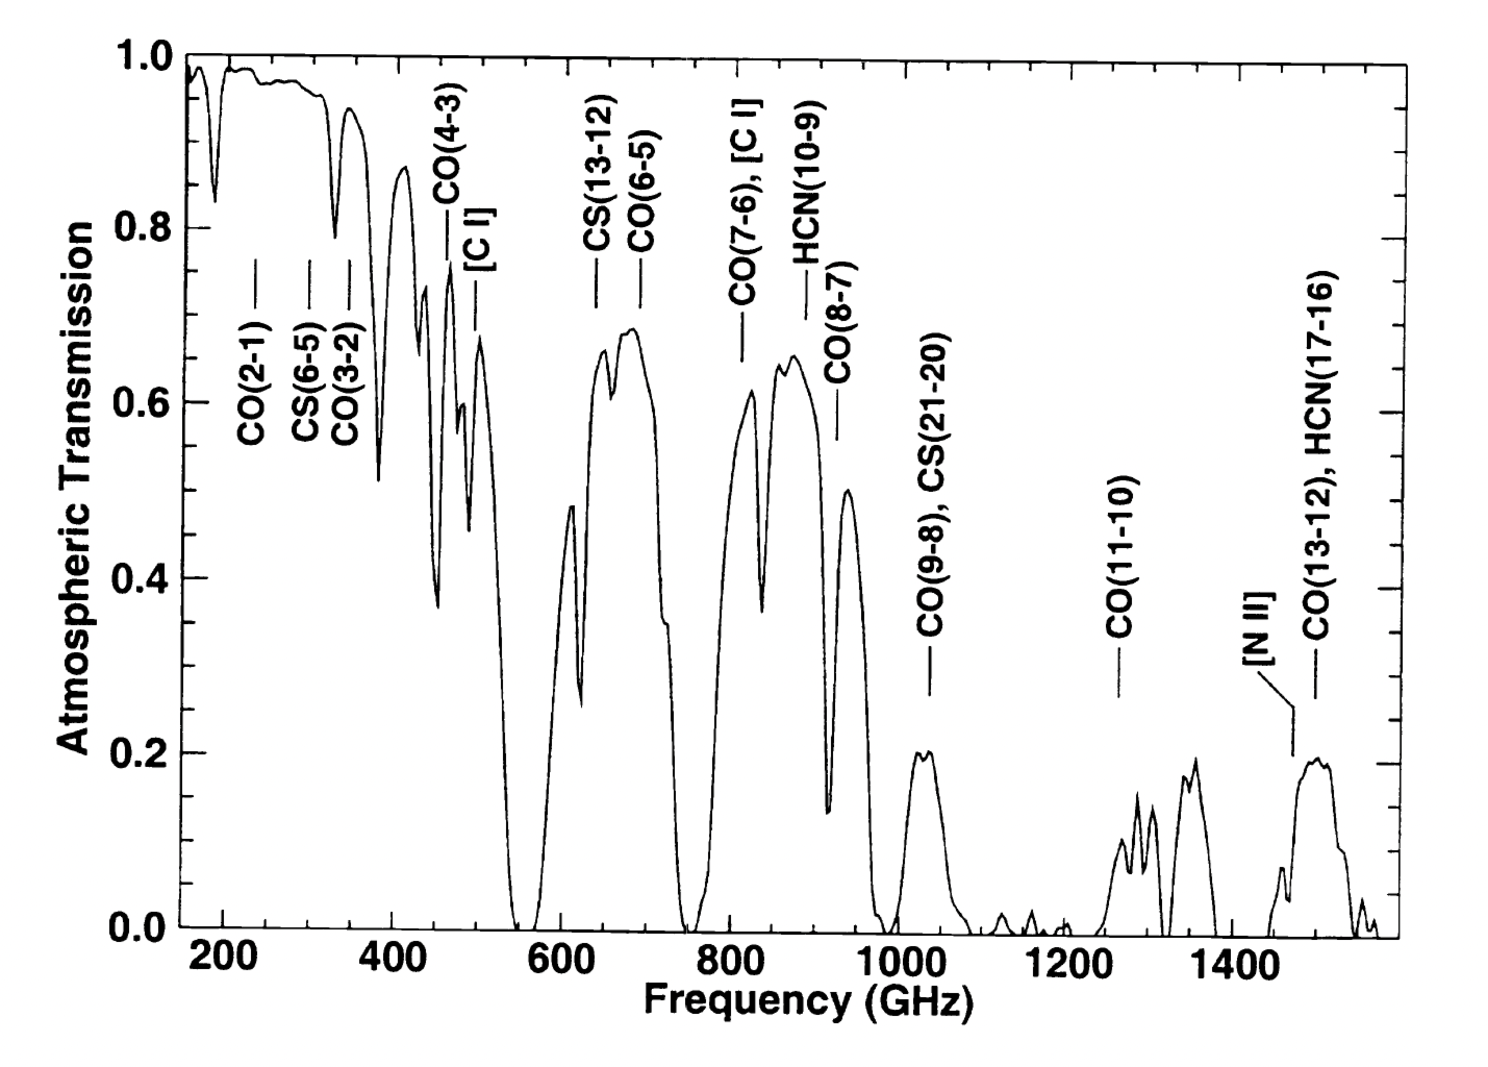
\includegraphics[angle=0.8, origin=c, width=0.8\columnwidth]{Figures/transmission.pdf}
	\caption[Atmospheric transmission of (sub-) mm wavelengths from Pampa la Bola]{The atmospheric transmission spectrum at (sub-)millimeter wavelengths as observed at Pampa la Bola ($4,800\,$m above sea level in Chile) and illustrated in \citealt{Matsushita_2000}. Overplotted are the locations of various CO, CI, CS, NII and HCN transition lines.}
	\label{fig:transmission}
\end{figure}

Let us briefly return to the Hubble Deep Field, shown in Figure \ref{fig:hubble_deep_field}. We saw that the field contains a wide variety of galaxies with different morphologies, ages and colours. An important point of note is that there are a number of massive ($>10^{10}\,M_\odot$) elliptical galaxies that can be observed in the local Universe. These galaxies are typically characterized by old stellar populations, limited cold gas and dust, and red colours. The $z = 0$ ages of these galaxies suggest that they had already formed their stellar mass at high redshift (e.g. \citealt{Gallazzi_2005, Thomas_2005}), implying that at some point in the past, they must have been rapidly forming stars and thus be incredibly bright. Without much luck finding these very active galaxies in the optical, the presence of highly dust-enshrouded galaxies with potentially starbursting phases, provides some credit to the idea that SMGs may be the progenitors of these massive elliptical galaxies in the Universe today, namely \textit{proto-ellipticals} (e.g. \citealt{Toft_2014, Valentino_2020b}). A better understanding of this population of galaxies may be key not only in our understanding of the obscured star formation at high redshifts, but also provide a target population in order to study the link between the early and local Universe.

In 1998, SCUBA was used to image the Hubble Deep Field at $450$ and $850\,\mu$m; the $850\,\mu$m data covering an area of approximately $9$ square arcminutes. At the time, the map of the Hubble Deep Field imaged with SCUBA, presented in \citealt{Hughes_1998}, was the deepest sub-mm map ever taken (a section with radius $100\,$arcsec from the $850\,\mu$m image center is shown in Figure \ref{fig:hubble_deep_field_scuba}). Many of the peaks in the image are a result of source confusion (Section \ref{sec:challenges}), but $5$ reliable sub-mm sources were identified. Despite a comparatively small number of detections compared to the same size area on the Hubble image, the total energy outputs are roughly the same. The brightest source, HDF850.1, is an exceptional example of the extreme nature of these sources. HDF850.1 has a star formation rate of $\sim 850\,M_\odot$yr$^{-1}$ (\citealt{Walter_2012}), which is comparable to the total number of stars we expect to be being formed in all the other galaxies in the optical image combined. Moreover, the incredibly dusty nature of this source means that an unambiguous counterpart at shorter wavelengths could not be identified, even in the deepest optical image of the Universe ever taken at the time. The identification of an optical/infrared counterpart has continued to be elusive with only a handful of studies making claims for having identified the galaxy producing the sub-mm emission, with much contention (e.g. \citealt{Dunlop_2004, Serjeant_2014, Sun_2023}).

\begin{figure}
    \centering
	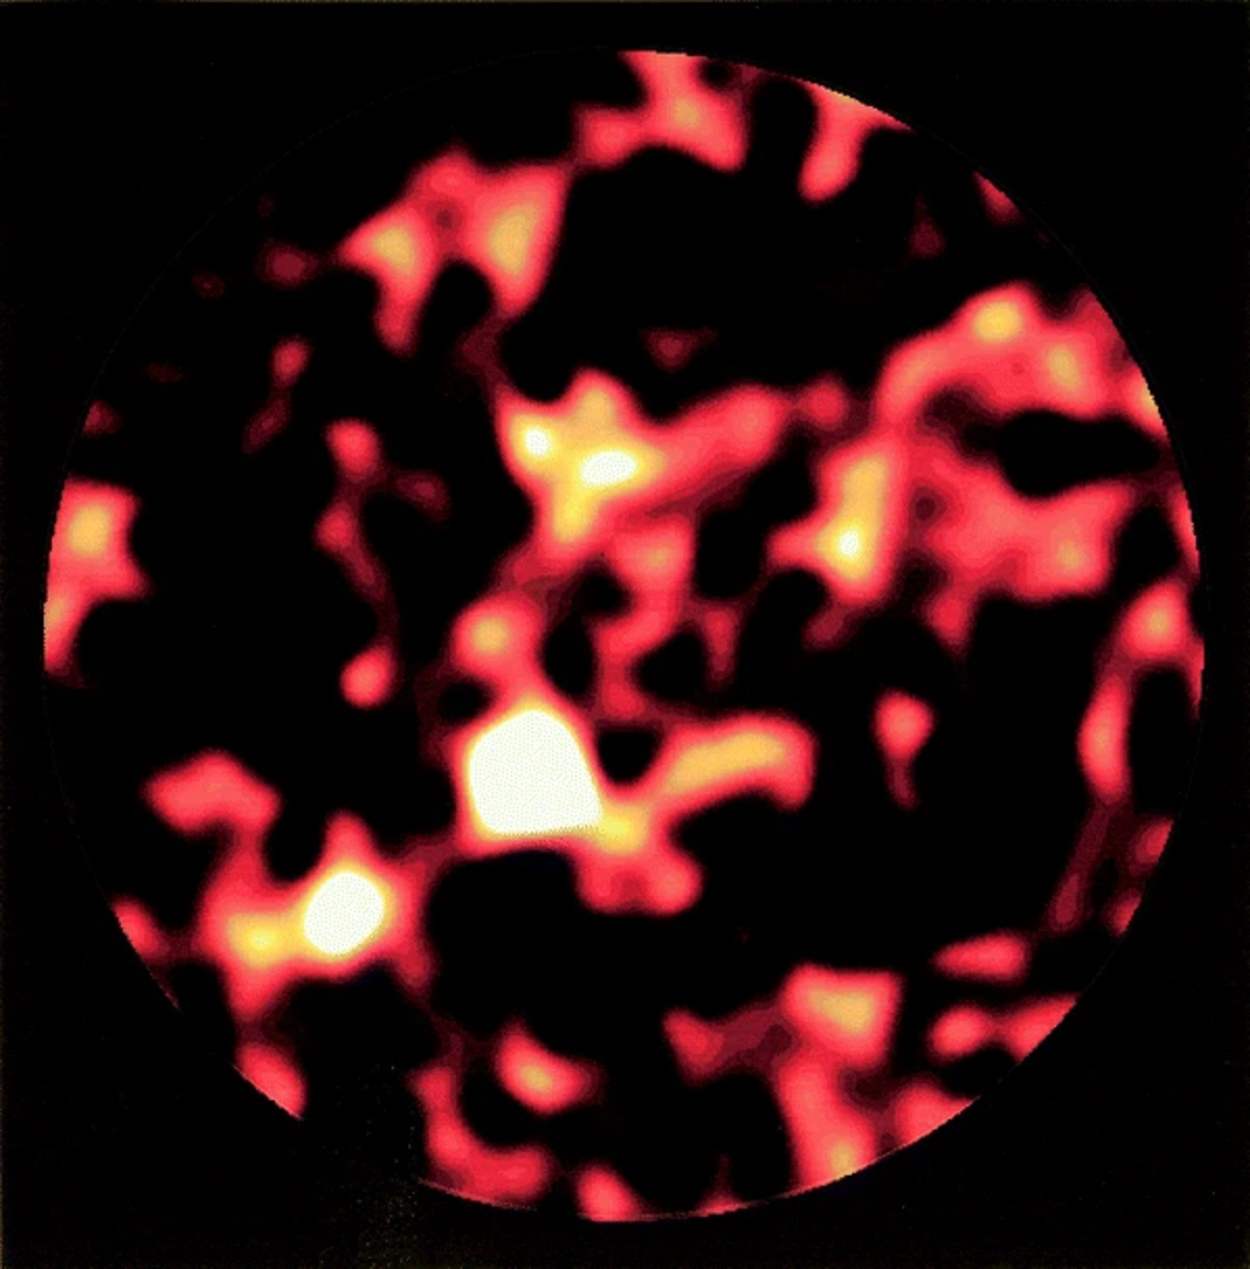
\includegraphics[width=0.8\columnwidth]{Figures/hubble_deep_field_scuba.pdf}
	\caption[Hubble Deep Field as captured by SCUBA on the JCMT]{The $850\,\mu$m map of the Hubble Deep Field taken with the SCUBA camera on the JCMT and presented in \citealt{Hughes_1998}. The image is of a patch of the field with a radius of $100\,$arcsec and shows $5$ statistically identified sub-mm galaxies.}
	\label{fig:hubble_deep_field_scuba}
\end{figure}

With continual improvement in the sensitvity of bolometer-arrays, samples of DSFGs detected at sub-mm wavelengths, particularly at $\sim 850\,\mu$m, have continually grown (e.g. \citealt{Borys_2003, Coppin_2006, Weiss_2009, Casey_2013, Geach_2017}). If we wish to observe these same galaxies at far-IR wavelengths closer to the peak of the dust emission we find that the atmospheric transmission falls to zero. These observations are especially vital in characterizing the properties of the dust in these galaxies; without observations constraining the peak of the dust emission basic properties like the mass and temperature of the dust are very hard to predict. The Balloon-borne Large Aperture Submillimeter Telescope (BLAST; \citealt{Devlin_2009}) was an ambitious project to overcome these observational constraints by launching a far-infrared telescope hanging from a high-altitude balloon. Above most of the Earth's atmosphere it was able to detect several hundred sources across several flights, but was limited by its large beamsize ($33$, $46$ and $66\,$arcsec at $250$, $350$ and $500\,\mu$m, respectively). Nevertheless, BLAST provided observations that filled in the gap that had been left by other instruments between the long wavelength \textit{Spitzer Space Telescope} bands (up to the $160\,\mu$m band) and the sub-mm wavebands.

\subsection{The \textit{Herschel Space Observatory}}

While BLAST was opening up this key region of the IR spectrum, a new spaceborne telescope was being prepared for launch. Initially called the \textit{Far InfraRed and Sub-millimeter Telescope} (FIRST) but subsequently changed to the \textit{Herschel Space Observatory} (\citealt{Pilbratt_2010}), \textit{Herschel} launched in May 2009 with a $3.5\,$m diameter primary mirror, making it the largest infrared space telescope prior to the launch of the \textit{James Webb Space Telescope} (JWST) on Christmas Day 2021. The mission built upon previous infrared space missions including the \textit{Infrared Astronomical Satellite} (IRAS; \citealt{Neugebauer_1984}), the \textit{Infrared Space Observatory} (ISO), \textit{Spitzer} and AKARI (\citealt{Murakami_2007}), by increasing the collecting area of the mirror and extending coverage to longer wavelengths that had never before been accessible from a space observatory. \textit{Herschel} covered a wide wavelength range from $55$ to $672\,\mu$m, and while its predecessors covered some of this broad part of the spectrum (for example, ISO observed in the wavelength range from $2.5$ to $240\,\mu$m and \textit{Spitzer} obtained imagery and spectra in the range $3$ to $180\,\mu$m), the improved resolution and sensitivity of \textit{Herschel} allowed for more detailed study of the cold dust in galaxies.

The operational wavelength range drives the science objectives of an instrument, in the case of \textit{Herschel}, this range corresponds to the peak continuum emission from bodies with temperatures between $\sim5$ and $50\,$K and the bright molecular and atomic emission lines from gases with temperatures between $10$ and several hundered K (\citealt{Pilbratt_2008}). The thermal radiation from dust grains dominate the emission observed in the \textit{Herschel} range, allowing us to observe star forming molecular clouds at the stellar level within the Galaxy and the integrated properties of actively star forming galaxies at high redshifts. The key science objectives of \textit{Herschel} were based on these capabilities, focusing on the formation and evolution of stars and galaxies and the interaction with the ISM. In particular, the main science drivers were: to survey the extragalactic and Galactic sky in order to measure the obscured star formation activity over cosmic time (Section \ref{sec:cosmic_star_formation_history}); to study the physics and chemistry of the ISM; and to understand the stellar and interstellar lifecycle from observational astrochemistry.

\textit{Herschel} had three instruments onboard: the \textit{Spectral and Photometric Imaging Receiver} (SPIRE; \citealt{Griffin_2010}); the \textit{Photodetector Array Camera and Spectrometer} (PACS; \citealt{Poglitsch_2010}); and the \textit{Herschel-Heterodyne Instrument for the Far-Infrared} (HIFI; \citealt{deGraauw_2010}). In the context of this Thesis, we shall be mainly focused on the photometric capabilities of PACS and SPIRE. PACS was operational as both an imaging photometer and an integral field spectrometer. The imaging photometer had three broadband photometric bands centered at $70\,\mu$m ($60 - 85\,\mu$m), $100\,\mu$m ($85 - 130\,\mu$m) and $160\,\mu$m ($130 - 210\,\mu$m), which could observe simultaneously at $160\,\mu$m and one of the $70$ or $100\,\mu$m bands. The beamsizes of the PACS instrument depended on the scan rate being used, but were typically of order $5$, $7$ and $12\,$arcsec at $70$, $100$ and $160\,\mu$m, respectively. The photometer's wavebands were ideally placed to study the peak of dust emission in local galaxies, which could be observed to a point source detection limit of $\sim 3\,$mJy in all three bands. SPIRE, also a spectrometer and an imaging photometer, operated at three waveband simultaneously centered at $250$, $350$ and $500\,\mu$m. Due to the longer wavelengths than PACS, the SPIRE beamsizes were larger at $18$, $26$ and $36\,$arcsec for $250$, $350$ and $500\,\mu$m, respectively, with confusion limits of approximately $5.8$, $6.3$ and $6.8\,$mJy (\citealt{Casey_2014b}). While the beamsizes are large, we note the marked improvement compared to the BLAST values mentioned earlier. Despite the larger beamsize, SPIRE mapping was more efficient than PACS mapping, making it particularly useful in imaging large areas of sky quickly. As a result, SPIRE has frequently been used to map large areas for extragalactic deep field surveys. Finally, HIFI, which does not feature in this Thesis, was a high resolution heterodyne spectrometer. Observing just a single pixel on the sky at a time, HIFI produced extremely detailed spectra of the molecules in a galaxy.

\subsection{\textit{Herschel} Surveys}

The launch of \textit{Herschel}, particularly with the mapping speed of the SPIRE instrument, allowed, for the first time, large scale surveys at wavelengths between $\sim 100$ and $500\,\mu$m. The rapid technological advancement in far-IR/sub-mm astronomy becomes clear when one compares the maps produced during \textit{Herschel}'s legacy programes with the first sub-mm images (e.g. Figure \ref{fig:hubble_deep_field_scuba}). As an example, Figure \ref{fig:gama9} shows one field, GAMA9, from the \textit{Herschel}-ATLAS project (which we shall describe in more detail in Chapter \ref{chapter:Data_Release_3}), which spans a total of nearly $54\,$deg$^2$. A preliminary data release, named the Science Demonstration Phase (SDP; \citealt{Ibar_2010, Rigby_2011, Pascale_2011}), focused on PACS and SPIRE photometry of one panel of the GAMA9 field (the second rectangular region from the left in Figure \ref{fig:gama9}), totalling $16\,$deg$^2$. This field contained almost $10,000$ galaxies and took \textit{Herschel} just $16$ hours to image. We compare this to the SCUBA Hubble Deep Field map, which took a total of $51$ hours to image an area approximately $600$ times smaller, detecting only $5$ secure sub-mm sources. This highlights the vast improvement in mapping speed and observing time required per source that had been made in the decade leading up to the launch of \textit{Herschel}.

\begin{figure}
    \centering
	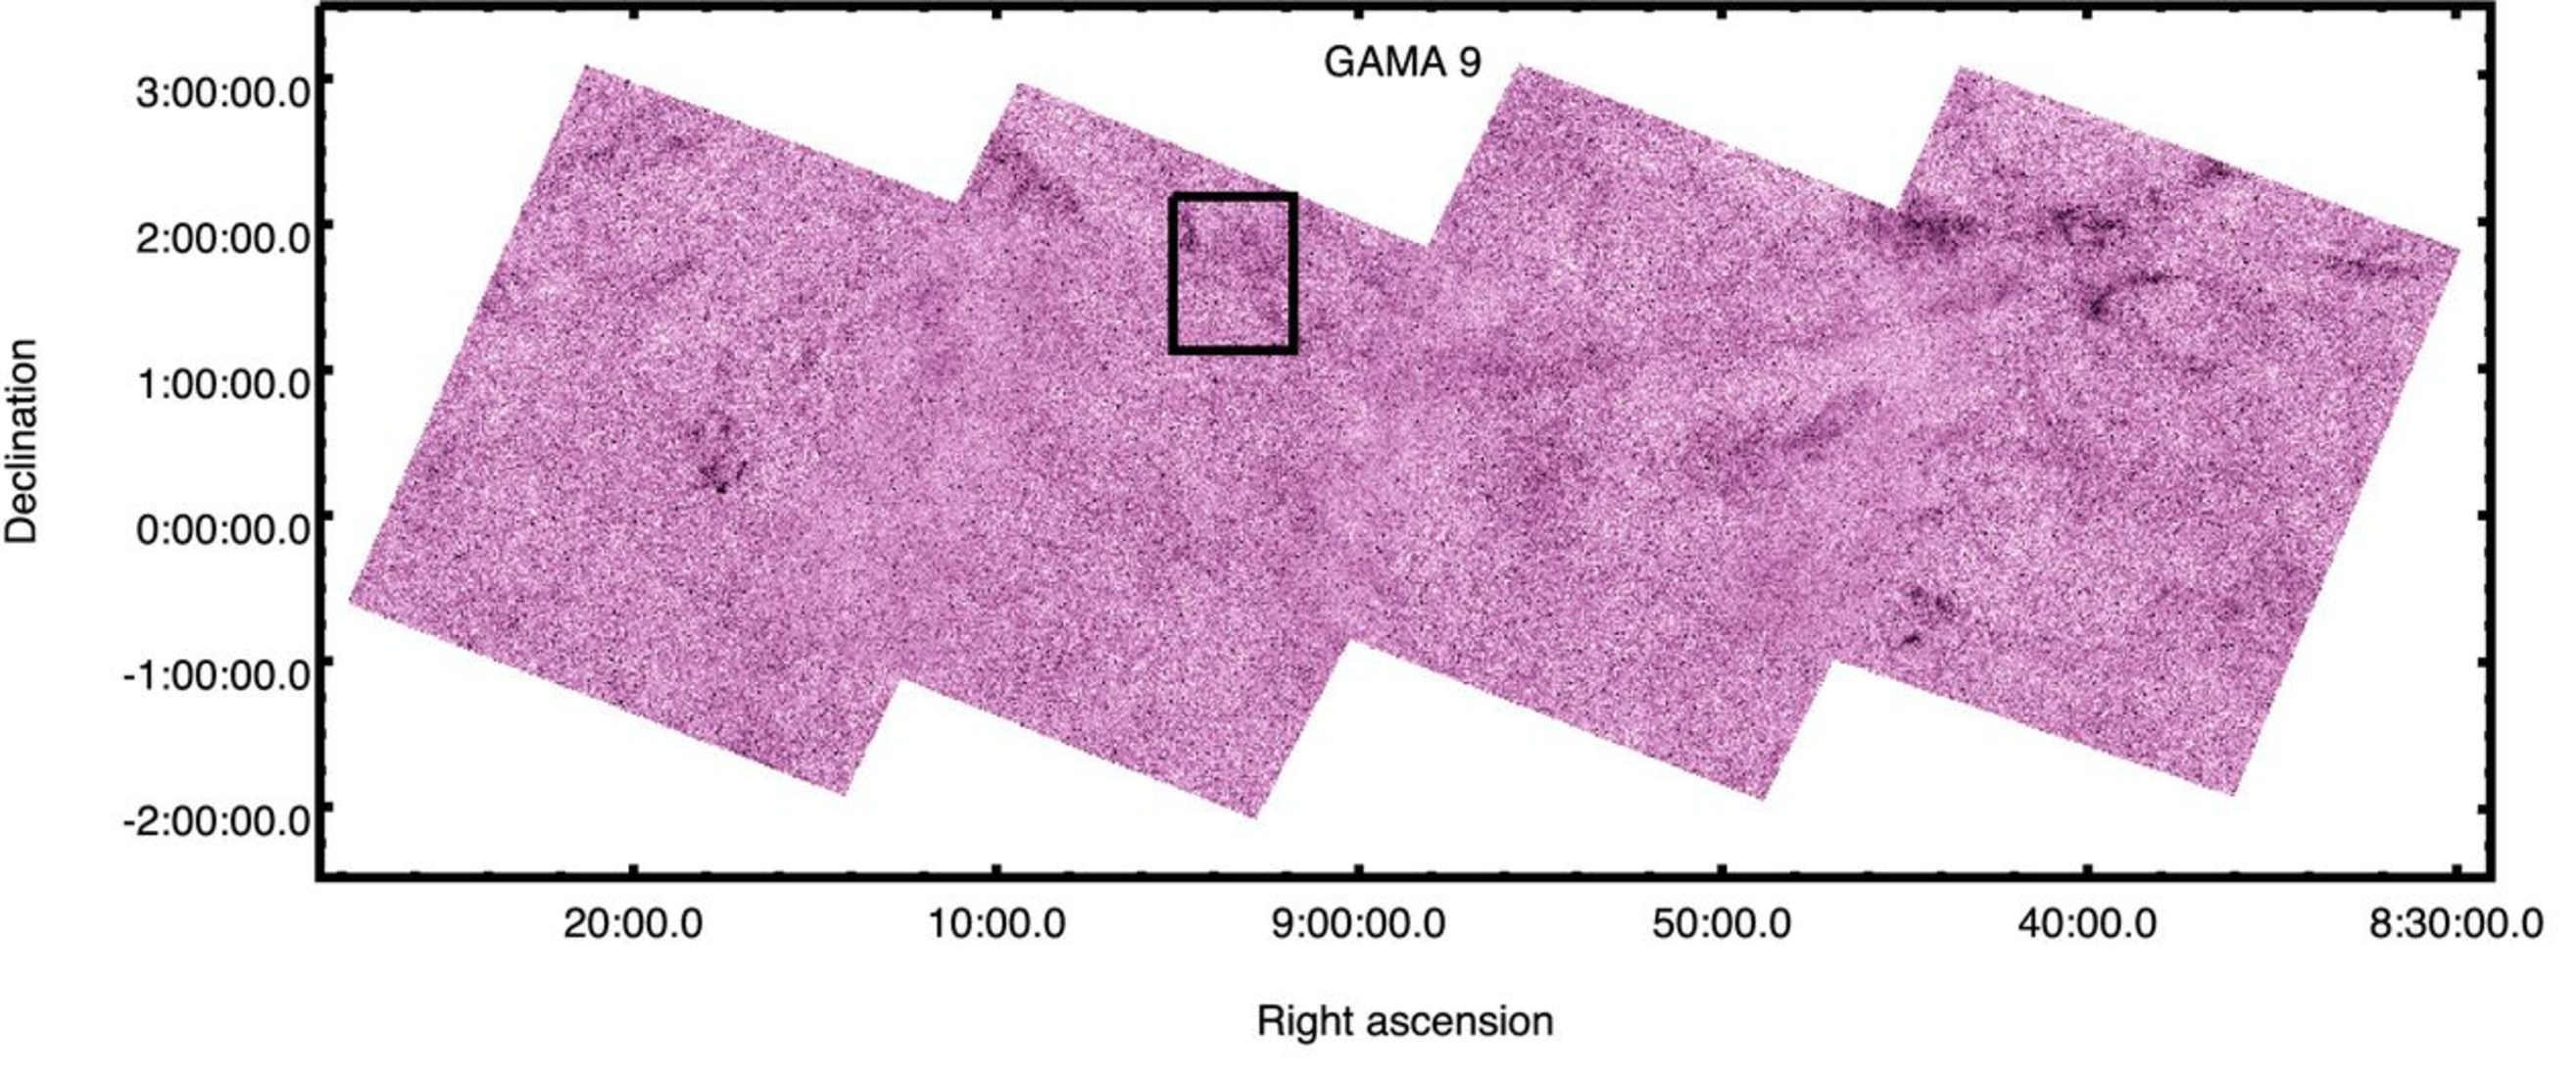
\includegraphics[width=0.9\columnwidth]{Figures/GAMA9.pdf}
	\caption[$250\,\mu$m map of the GAMA9 field of H-ATLAS]{The $250\,\mu$m image of the GAMA9 field of the \textit{Herschel}-ATLAS. The Science Demonstration Phase (SDP) of the H-ATLAS project observed the second rectangular region from the left, which has an area of approximately $16\,$deg$^2$. The total area of the GAMA9 field is approximately $54\,$deg$^2$. The figure is as presented in \citealt{Valiante_2016}.}
	\label{fig:gama9}
\end{figure}

In total, extragalactic surveys with \textit{Herschel} exceed $1,000\,$deg$^2$ in area. During this Thesis we will be mainly focused on two \textit{Herschel} surveys, the \textit{Herschel}-Astrophysical Terahertz Large Area Survey (H-ATLAS; \citealt{Eales_2010}) and the \textit{Herschel} Multi-tiered Extragalactic Survey (HerMES; \citealt{Oliver_2012}). Both surveys will be described in detail, H-ATLAS in Chapter \ref{chapter:Data_Release_3} and HerMES in Chapter \ref{chapter:Radio_Identifications}. Figure \ref{fig:herschel_surveys} shows the area of various \textit{Herschel} surveys against the point source depth, showing that HerMES consists of a range of shallow and wide fields and deep and narrow fields, and that the \textit{Herschel}-ATLAS was the largest extragalactic survey in open time, spanning approximately $660\,$deg$^2$ in total. H-ATLAS was designed to be a shallow survey that could rapidly map a large area of sky, detecting hundreds of thousands of galaxies from their cold dust emission. This survey forms the cornerstone of this Thesis, allowing us to measure the evolution of the dusty ISM for a large number of galaxies in the past several billion years of cosmic history.

\begin{figure}
    \centering
	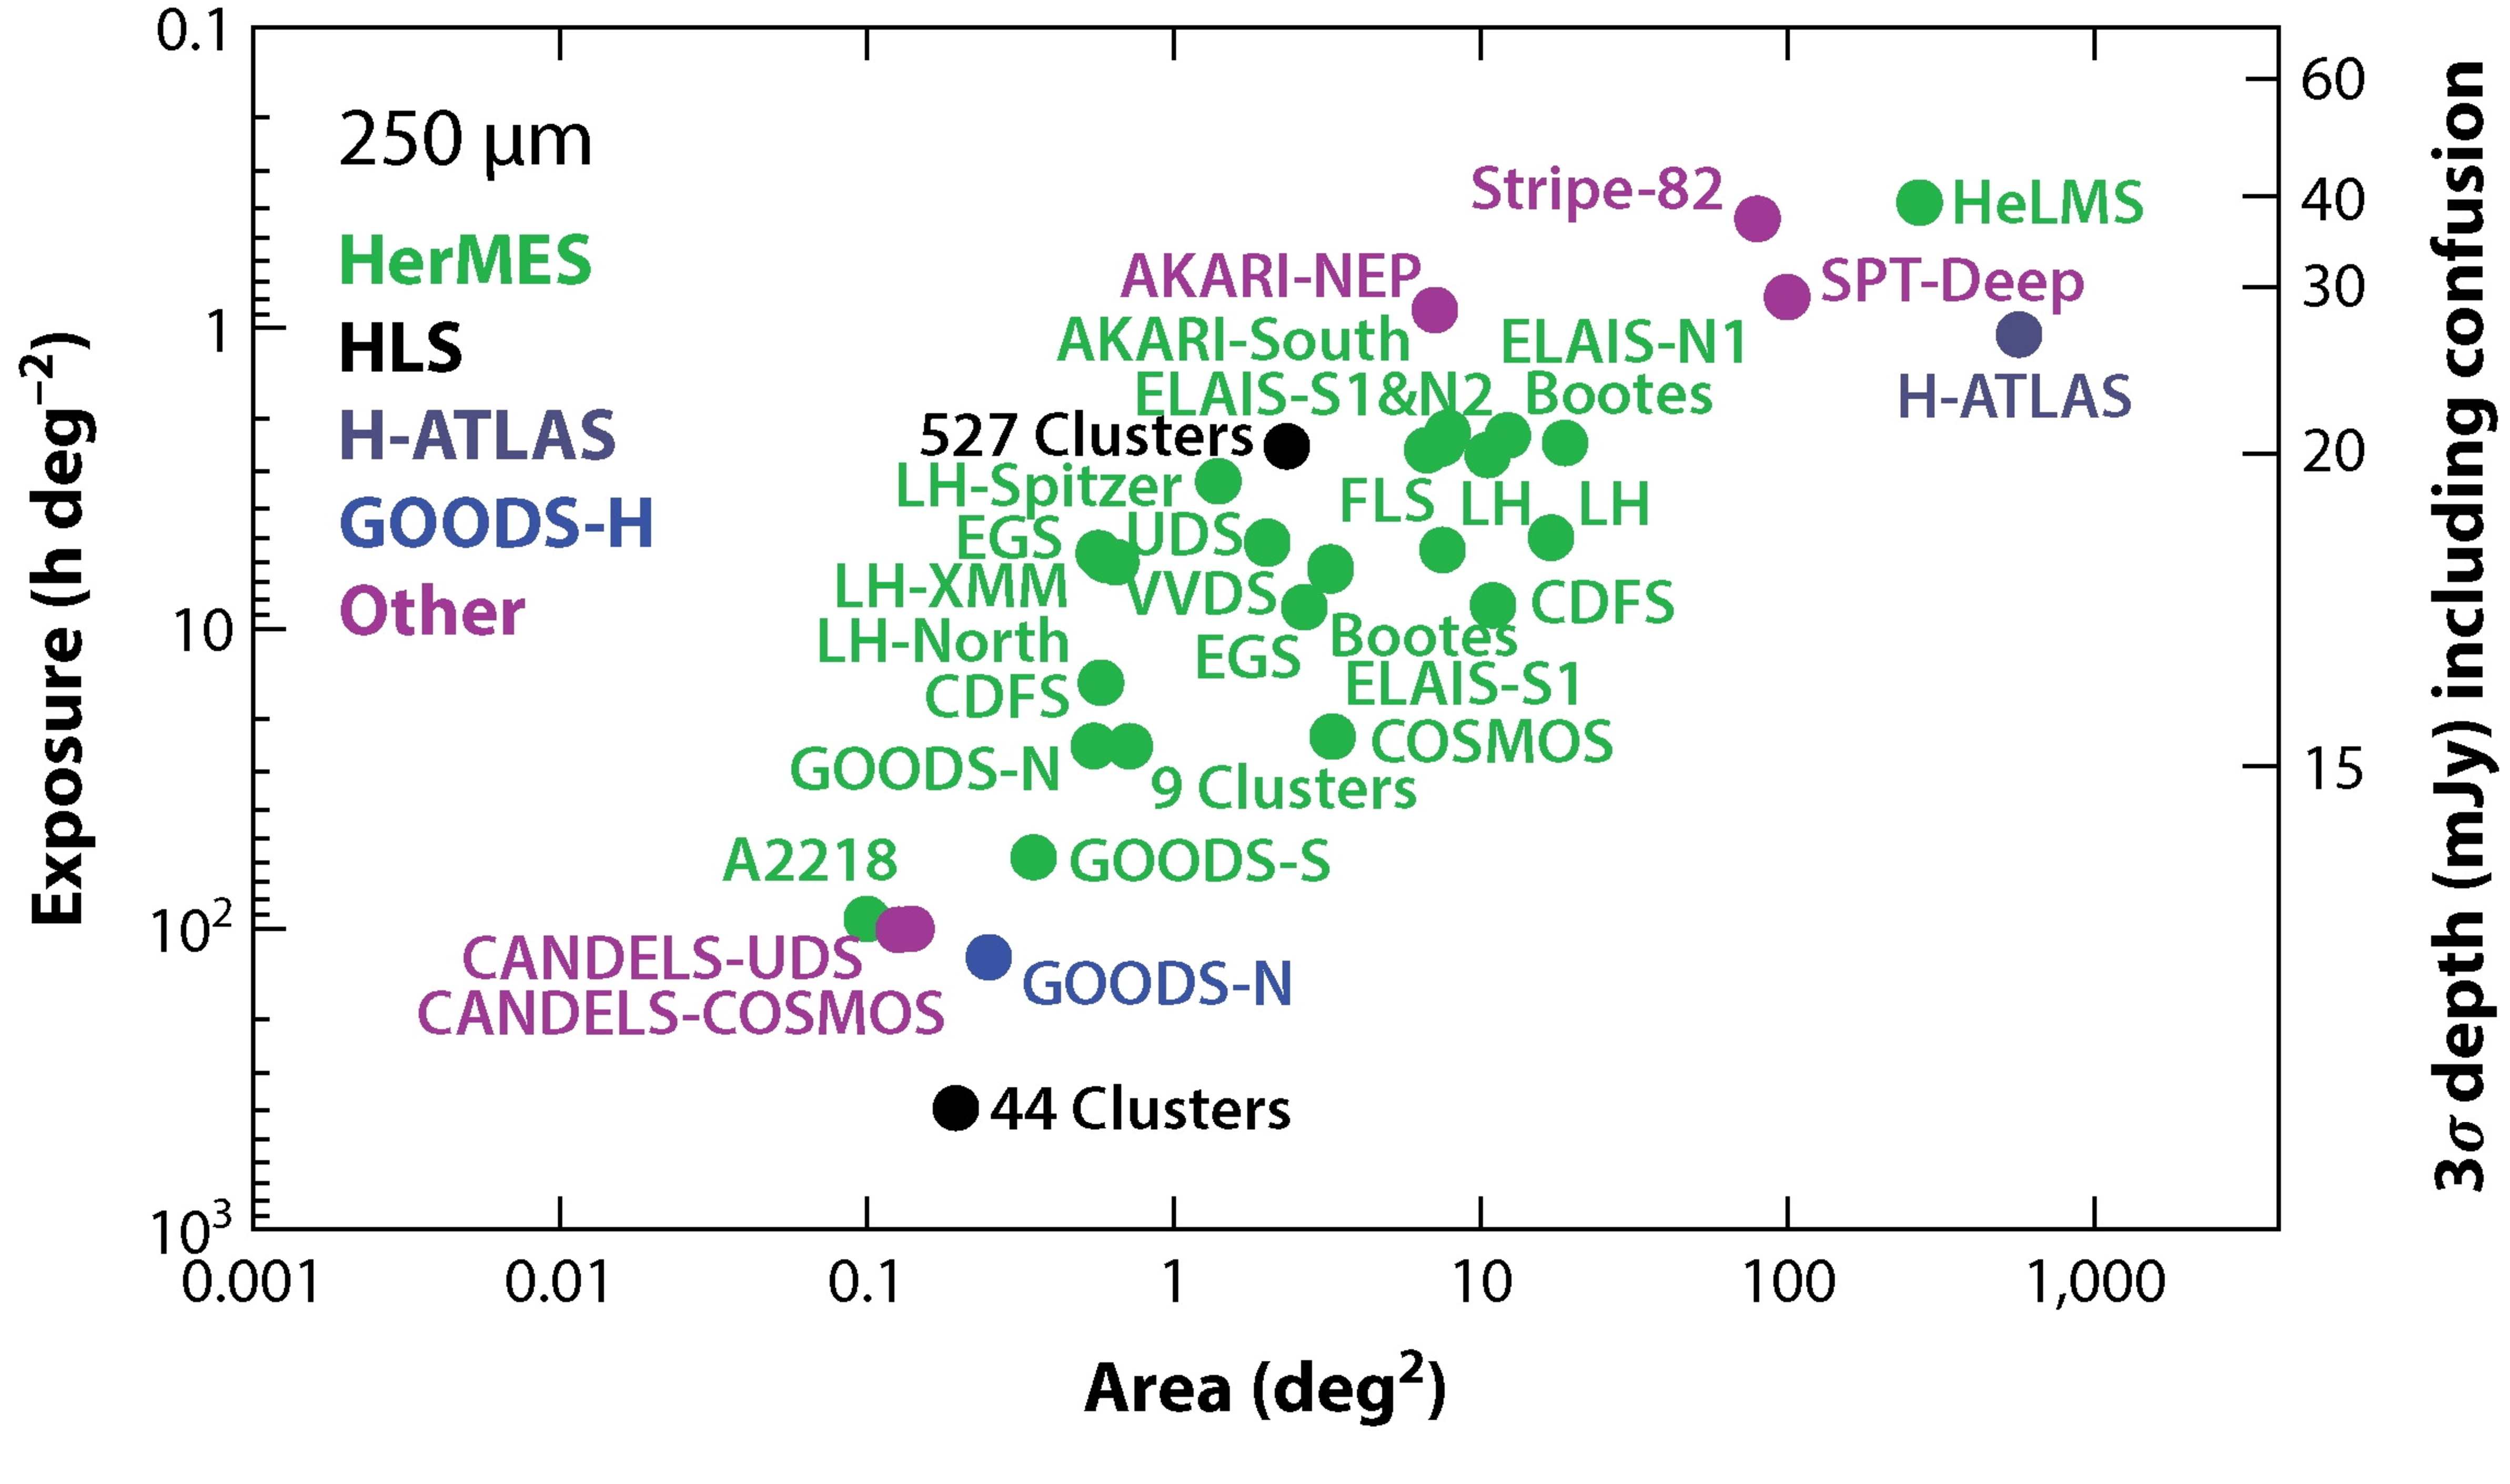
\includegraphics[width=0.9\columnwidth]{Figures/herschel_surveys.pdf}
	\caption[Survey area against point source depth for extragalactic \textit{Herschel} surveys]{The survey area against the point source depth of a selection of extragalactic surveys at $250\,\mu$m with \textit{Herschel}, as presented in \citealt{Lutz_2014}. The figure shows the fields that form the following surveys: the \textit{Herschel} Multi-tiered Extragalactic Survey (HerMES, green circles); \textit{Herschel} Lensing Survey (HLS, black circles); \textit{Herschel}-Astrophysical Terahertz Large Area Survey (H-ATLAS, dark blue circles) and Great Observatories Origins Deep Survey - Herschel (GOODS-H, blue circles).}
	\label{fig:herschel_surveys}
\end{figure}

\section{Challenges in Identifying DSFGs and their Multiwavelength Counterparts}
\label{sec:challenges}

The reason why the far-IR and sub-mm regions of the electromagnetic spectrum have been elusive to astronomers until very recently is partly due to the difficulties in constructing the instruments and telescopes required for these wavelengths. As we have seen in Section \ref{sec:first_submm_galaxies}, one obstacle is the atmospheric absorption caused by water vapour in the Earth's atmosphere, requiring far-IR and sub-mm telescopes to be located at high-altitude sites or in space. Adding to this, the cameras themselves are not like the typical photodetectors that may be used at other wavelengths, but instead are \textit{bolometers} that detect infrared radiation by measuring the increase in temperature when radiation gets absorbed (\citealt{Woodcraft_2009}). The first bolometer was built by Samuel Pierpont Langley in 1880 (\citealt{Langley_1880}), and were initially limited to single-pixel devices. The breakthrough for sub-mm astronomy came with the first bolometer cameras in the 1990s, which linked multiple bolometers together to make a multi-pixel camera. However, the difficulty in applying these newly discovered bolometer cameras to observing thermal radiation from dust is that the thermal radiation from the instruments themselves will cause substantial noise. This requires operating them at ultra-low temperatures (typically no more than $\sim 300\,$mK). Most sub-mm telescopes thus carry coolant to cryogenically cool the instruments, which means that the lifespan of the telescope is predetermined (\textit{Herschel} was operational for four years between 2009 and 2013, during which time its liquid Helium reserve cooled the detectors to $\sim 300\,$mK and the rest of the observatory to $1.7\,$K). Moreover, for a spaceborne observatory, the size of the primary mirror is restricted by the limitations of launching the telescope to space (although some novel approaches like the folding mirrors of JWST have increased the light collecting area we have in space). This is problematic given that the resolution of a telescope is dependent on the diameter of the primary mirror, $D$, and the observing wavelength, $\lambda$, according to $\theta = 1.22\lambda/D$. The combination of the long wavelength sub-mm bands and the smaller mirrors of spaceborne telescopes means that the angular resolution of sub-mm telescopes are typically poor.

The result of low angular resolution is source confusion. This occurs when more than one source is present in the observing beam due to the faint signals from unresolved sources (\citealt{Condon_1974}). As fainter objects far outnumber brighter objects, far-IR/sub-mm surveys have a minimum flux density below which you become confusion limited and the number of DSFGs that can be observed is highly dependent on them being high significance detections in order to avoid counting spurious peaks in the noisy maps. This limitation is emphasized by an effect that was earlier presented as an advantage of the far-IR/sub-mm bands: the negative K-correction. These wavebands are particularly susceptible to source confusion because the negative K-correction causes distant galaxies to appear in images with comparable brightness to nearer galaxies, meaning a greater chance of multiple faint objects being present within a single beam.

The optical to IR counterparts of our DSFGs are used to derive photometric redshifts as well as basic properties such as the stellar mass and star formation rates (from dust-unobscured star formation) of our dusty galaxies. Indeed, the multiwavelength view of a galaxy is important in obtaining a full picture of the galaxy population and their evolution. However, characterizing our galaxies at other wavelengths could lead to a biased view of the population if we cannot localize the counterparts for a complete sample of DSFGs. The large beamsize of single-dish sub-mm observations means that these sources typically have positional uncertainties of several arcseconds (which increases with the source's flux density) and the number of possible counterparts that can be observed in the vicinity of the location of the dust emission can be many. Figure \ref{fig:viking_cutout} shows a region $12\times12\,$arcsec around a \textit{Herschel} source detected in H-ATLAS (black cross). The figure shows the VISTA Kilo-degree Infrared Galaxy (VIKING) survey $K_s$ band image of the same region, showing two potential near-IR counterparts (highlighted red and blue). Such a scenario where locating the true source of the dust emission is not trivial, is not uncommon. The most reliable way of refining the position of the source is to use interferometric observations with the likes of the Atacama Large Millimeter/submillimeter Array (ALMA) to secure the position to approximately arcsec resolution, however, this is impractical for large surveys, and to crossmatch all our far-IR/sub-mm sources with their multiwavelength counterparts, without the use of expensive, targeted observations, we must find alternative methods that directly match to our low resolution observations.

\begin{figure}
    \centering
	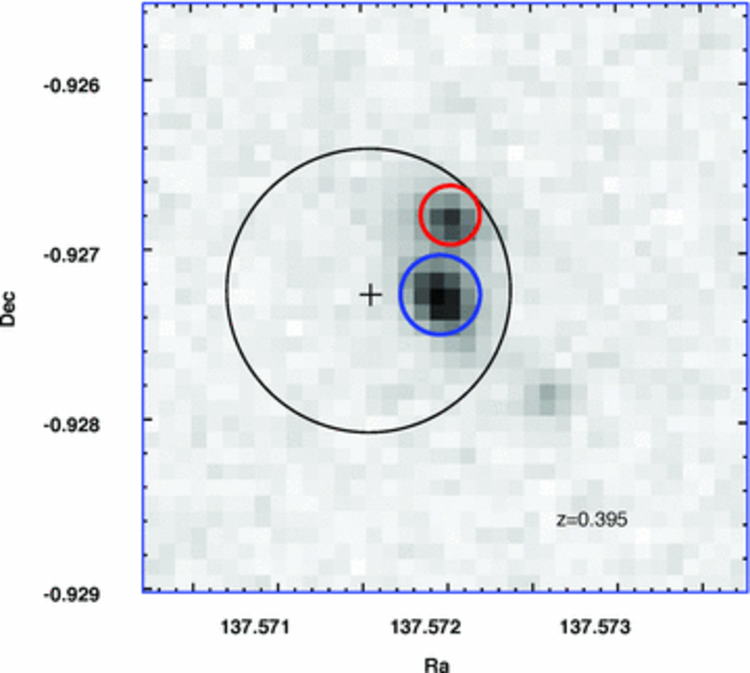
\includegraphics[width=0.8\columnwidth]{Figures/viking_cutout.pdf}
	\caption[VISTA-VIKING cut-out of H-ATLAS J091017.1-005538]{A VISTA-VIKING cut-out of H-ATLAS J091017.1-005538 in the $K_s$ band ($2.15\,\mu$m) from \citealt{Fleuren_2012}. The location of the far-IR emitting region is indicated by a black cross with a $2\sigma = 2.9\,$arcsec positional uncertainty for this source represented by a black circle. Two potential near-IR counterparts are highlighted by red and blue circles; a third with negligible probability of being the true association can be seen outside the $2.9\,$arcsec radius.}
	\label{fig:viking_cutout}
\end{figure}

\section{Outline of Thesis}

In this Thesis we study several open questions about interstellar dust in active star forming galaxies. We study a sample of \textit{Herschel} detected galaxies at $z < 1$ and derive the evolution of their dust content, spanning the past $8$ billion years, closing in on the peak in cosmic star formation. At higher redshifts, we study the dust properties of a sample of DSFGs to test whether the common assumption of extragalactic studies, that the properties of dust are the same at all epochs, holds true by comparison with local values. Finally, we identify a sample of \textit{Herschel} galaxies for which we have robust UV-IR spectra to understand the role that they play in the dust obscured star formation activity of the Universe and their stellar mass assembly histories. The following is an outline of each Chapter:

\begin{itemize}
	\item In Chapter \ref{chapter:Data_Release_3}, we introduce the \textit{Herschel}-ATLAS survey and conduct a thorough Bayesian analysis, namely the Likelihood Ratio method, to identify near-IR counterparts to \textit{Herschel} sources in the South Galactic Pole (SGP) field. We also present a new method in which to predict the number of potential strong and weak gravitational lensing events within a blank \textit{Herschel} field, with no constraints from a minimum \textit{Herschel} flux density. The majority of the research from this chapter can be found in \citealt{Ward_2022}.
	\item In Chapter \ref{chapter:Dust_Mass_Functions}, we use the SGP sample from the previous chapter to measure the dust mass function (DMF) from $\sim80,000$ galaxies out to $z = 1$. We use our DMFs to derive the cosmic dust mass density over the past $8\,$Gyr and compare the evolution in the dust content of the Universe with the star formation rate density. The work estimating the dust temperatures of H-ATLAS galaxies is used in \citealt{Eales_2024}.
	\item In Chapter \ref{chapter:Dust_Evolution}, we present two samples of DSFGs that span redshifts between $z = 2$ and $z = 6$, one \textit{Herschel} selected as part of the \textit{Herschel Bright Sources} (HerBS) sample, and the other sample selected at $1.4\,$mm as part of the South Pole Telescope -- Sunyarv-Zel'dovich survey. Together, a total of approximately $100$ galaxies are used to predict the average dust properties of high redshift star forming galaxies, which we compare with local samples to test whether dust takes the same form at all times of cosmic history. The research from this chapter is presented in Ward et al., submitted.
	\item In Chapter \ref{chapter:Radio_Identifications}, we turn to the \textit{Cosmic Evolution Survey} (COSMOS) where approximately $10,000$ \textit{Herschel} galaxies have been observed as part of HerMES, along with $\sim10,000$ VLA sources at $3\,$GHz. We make use of the well-studied relationship between the far-IR and radio emission of star forming galaxies to identify highly probable radio counterparts which, with their good astrometric precision, allows for the unambiguous matching with multiwavelength associations. With exceptional coverage across the UV to far-IR spectrum for a large sample of \textit{Herschel} galaxies, we investigate their evolutionary state and the stellar mass assembly history of such galaxies.
	\item In Chapter \ref{chapter:Conclusion}, we provide a summary of our key findings from the Thesis and present potential avenues for future studies related to the research presented herein.
\end{itemize}

Through this work we attempt to answer the following questions; which we shall return to in our closing discussion. How has the dust content of galaxies evolved to the present day? Are the dust properties of galaxies the same at all cosmic epochs? And in what evolutionary stage do we observe dust-enshrouded, IR-bright galaxies; do they provide the link to the massive systems we observe in the local Universe today?

